This chapter will present the checks, tests and validations of the
BANFF fit using the MC simulation as input. The test using the weighted
MC as the data is referred as an Asimov\footnote{An Asimov data refers replacing the ensemble of simulated data sets
by a single representative one.} data fit\cite{Cowan:2010js}. There next are two other validation
tests that use two different data sets that have altered events weights
(reweighted) compared to the MC. These are referred to as fake data
sets.

The chapter is presented in the following order. The first topic is
the Asimov data fit discussed in \prettyref{sec:Asimov-Data-Fit}.
The following section explores the results of the two fake data fits
in \prettyref{sec:Fake-Data-Fits}. A chapter summary is provided
in \prettyref{sec:ValidationSummary}.


\section{Asimov Data Fit\label{sec:Asimov-Data-Fit}}

Asimov data refers to replacing the ensemble of simulated data sets
by a single representative one\cite{Cowan:2010js}. In this analysis,
this involves fitting the MC data set to itself for the primary purpose
of checking the closure of the fitting framework. The Asimov set is
produced with the same models as is implemented in the fitter and
has all parameters set to their prior central values as defined in
\prettyref{chap:P0DinBANFF}. Instead of statistically sampling from
the MC, which can insert statistical variations into the fit, the
Asimov data set is created by scaling the set down to the full T2K
POT with additional finer corrections like flux and cross section
weights. The prefit correlation matrix is shown in \prettyref{fig:Complete-prefit-correlation}.

\begin{figure}
\begin{centering}
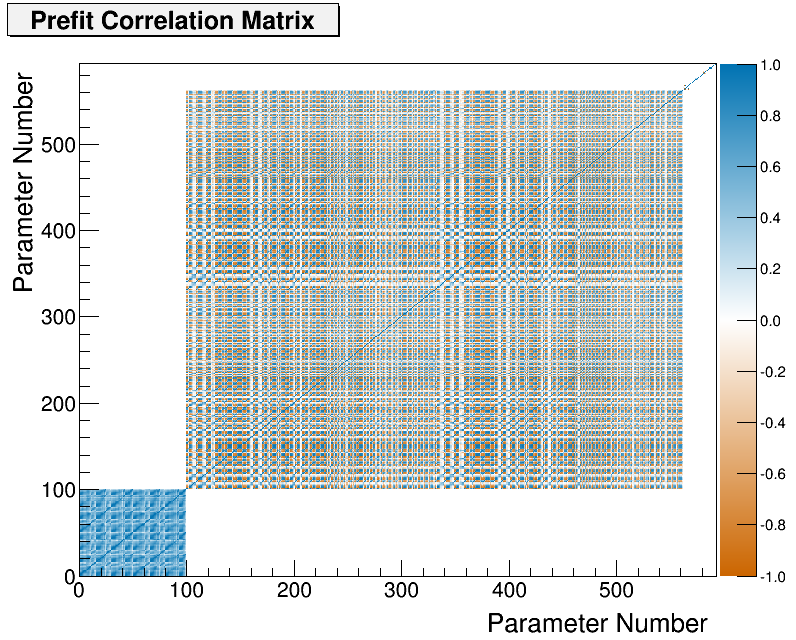
\includegraphics[width=0.95\textwidth]{Chapters/Figures/Validation/Asimov/corr_pref}
\par\end{centering}
\caption[Complete Prefit Correlation Matrix for the BANFF Fit.]{Complete prefit correlation matrix for the BANFF fit. The first 100
parameters are the flux bins. Between 100 and 561 are the bin normalization
parameters. Finally 562 through 592 are the cross section parameters.
\label{fig:Complete-prefit-correlation}}

\end{figure}

In addition to running an Asimov fit, other metrics were examined
in the Asimov set. Shown first is a comparison of the event rates
before and after applying weights to the MC. Next is an examination
of the cross section weight functions. Finally is a set of scans of
the test statistic space to check that the sample and penalty terms
are behaving as expected. Then the Asimov data set fit is examined.


\subsection{Event Rate}

Shown in \prettyref{tab:eventtable} are the event rates for the various
samples for the Asimov fit. The data events column refers to real
T2K data collected in ND280. The proceeding columns refer to MC events
only after applying different weights. The POT weight is a gross normalization
that scales the MC event rate to the data rate. The other weights,
which were discussed in \prettyref{chap:BANFF-Likelihood}, are the
flux, cross section, and detector corrections. As expected, we see
that applying the POT weight scales the MC event rate close to that
of the data. The other weights are fine tuning corrections to the
rate from known systematics like flux and cross sections. The set
of samples after applying all the weights is referred to as Asimov
data set.

\newpage{}

\begin{landscape}

\begin{table}
\caption[Event Rate Table for Asimov Set]{Event rate table for Asimov set. The ``Raw MC'' column refers the
number of events in the sample from the nominal MC prediction without
any weights applied. From left to right, applications of weights are
applied to understand their affect on the samples. The ``POT only''
column refers to applying the POT weight to all events. Columns with
``POT+Flux'', ``POT+xsec'', and ``POT+Det'' refer to applying
the POT weight together with the flux, cross section, and detector
weights, respectively. The ``Prefit'' column has the POT, flux,
cross section, and detector (POT+Flux+xsec+Det) weights all multiplied
together. \label{tab:eventtable}}

\centering{}\begin{tabular}{lccccccc}
\toprule
Sample & Data   & Raw MC & \multicolumn{4}{c}{Application of weights} & Prefit  \\ 
name   & events & events & POT only & POT+Flux  & POT+xsec  & POT+Det &  POT+flux+xsec+Det \\
\midrule
\midrule
$\nu_\mu$ 1-Trk Wtr &  27151.00 &  526226.00 &  26270.98 &  28766.86 &  24222.45 &  26286.14 &  27327.94\\ 
$\nu_\mu$ N-Trks &  31013.00 &  529538.00 &  26708.61 &  31464.27 &  26267.19 &  26708.74 &  31098.20\\ 
$\overline{\nu}_\mu$ RHC 1-Trk &  8779.00 &  176007.00 &  9152.04 &  9365.78 &  8321.76 &  9161.91 &  8461.37\\ 
$\overline{\nu}_\mu$ RHC N-Trks &  4613.00 &  93132.00 &  4876.93 &  5014.74 &  4652.01 &  4876.81 &  4802.12\\ 
$\nu_\mu$ RHC 1-Trk &  3502.00 &  56861.00 &  2933.20 &  3182.20 &  2747.29 &  2938.29 &  3025.76\\ 
$\nu_\mu$ RHC N-Trks &  5424.00 &  85599.00 &  4460.10 &  4988.89 &  4413.01 &  4464.45 &  4956.19\\ 
$\nu_\mu$ 1-Trk Air &  23504.00 &  309373.00 &  23383.39 &  25319.17 &  21594.49 &  23402.63 &  23603.03\\ 
$\nu_\mu$ N-Trks &  32736.00 &  371986.00 &  28495.10 &  33255.58 &  27822.42 &  28505.66 &  32302.08\\ 
$\overline{\nu}_\mu$ RHC 1-Trk &  6681.00 &  75374.00 &  7374.13 &  7512.47 &  6732.25 &  7381.37 &  6767.79\\ 
$\overline{\nu}_\mu$ RHC N-Trks &  4437.00 &  47951.00 &  4689.16 &  4820.43 &  4446.52 &  4690.57 &  4544.72\\ 
$\nu_\mu$ RHC 1-Trk &  2324.00 &  20943.00 &  2049.01 &  2198.46 &  1916.33 &  2052.56 &  2067.12\\ 
$\nu_\mu$ RHC N-Trks &  4801.00 &  42098.00 &  4119.63 &  4586.22 &  4050.71 &  4122.39 &  4567.72\\ 
\midrule
Total &  154965.00 &  2335088.00 &  144512.28 &  160475.06 &  137186.41 &  144591.53 &  153524.03\\
\bottomrule
\end{tabular}

\end{table}

\end{landscape}

\newpage{}


\subsection{One Sigma Variation of Cross Section Parameters}

It is difficult to predict the impact of cross section parameters
variations in the BANFF fit since the fit samples contain many interaction
modes themselves. In particular, a single parameter variation can
also be explained by many parameters individually varied. To understand
the effect of the cross section parameter variations on the fit samples,
each cross section parameter was varied by $\pm1$ standard deviation.
This also ensures the spline weight functions, which are generated
for each event prior to the BANFF fit, are functioning properly. The
results of the variations are shown in Appendix \prettyref{app:NSigmaVariations}.


\subsection{Log-Likelihood Scans}

Log-likelihood scans of the sample and penalty terms were examined
in the Asimov data set. The results of the scans are shown in \prettyref{fig:TestStatisticScans}
with comparisons between the $\pod$-only samples and FGD-only samples
shown. It can be seen that the $\pod$-only data has similar sensitivity
and shape dependence on the flux parameters to that of the FGD-only
data. Also observed is that the penalties are the identical for both
$\pod$- and FGD-only sets and parabolic in shape as expected since
the penalties are modeled using a Gaussian. The complete set of scans
is contained in Appendix \prettyref{app:Log-Likelihood-Sample-Scans}
and Appendix \prettyref{app:Log-Likelihood-Penalty-Scans}.

\begin{figure}
\begin{centering}
\subfloat[Flux normalization \textbf{$b_{3}$ }$\Delta\chi_{\text{LLR}}^{2}$
scan]{\begin{centering}
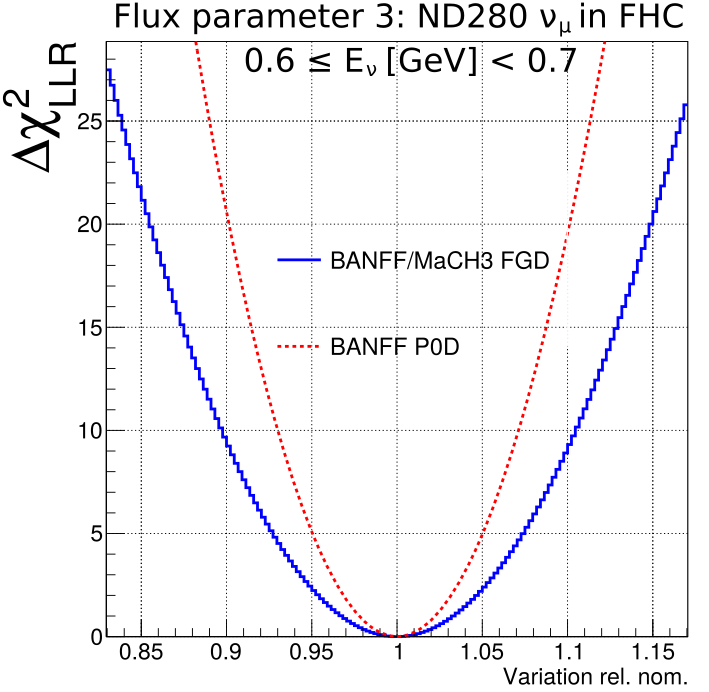
\includegraphics[width=0.45\textwidth]{Chapters/Figures/Validation/Asimov/Flux03Sample}
\par\end{centering}
}\subfloat[FSI low energy inelastic shape location $\Delta\chi_{\text{LLR}}^{2}$
scan]{\begin{centering}
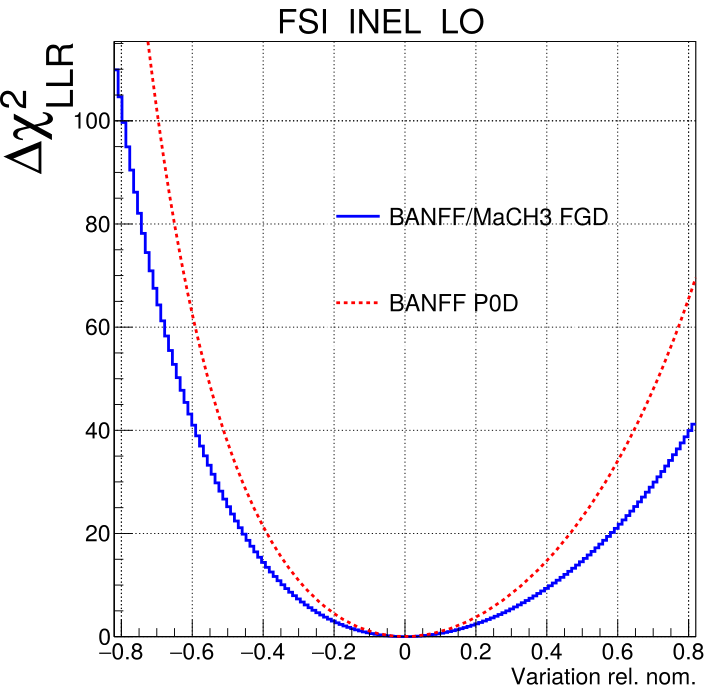
\includegraphics[width=0.45\textwidth]{Chapters/Figures/Validation/Asimov/FSIINELLOSample}
\par\end{centering}
}
\par\end{centering}
\begin{centering}
\subfloat[Flux normalization \textbf{$b_{3}$ }$\Delta\chi_{\text{Flux}}^{2}$
scan]{\begin{centering}
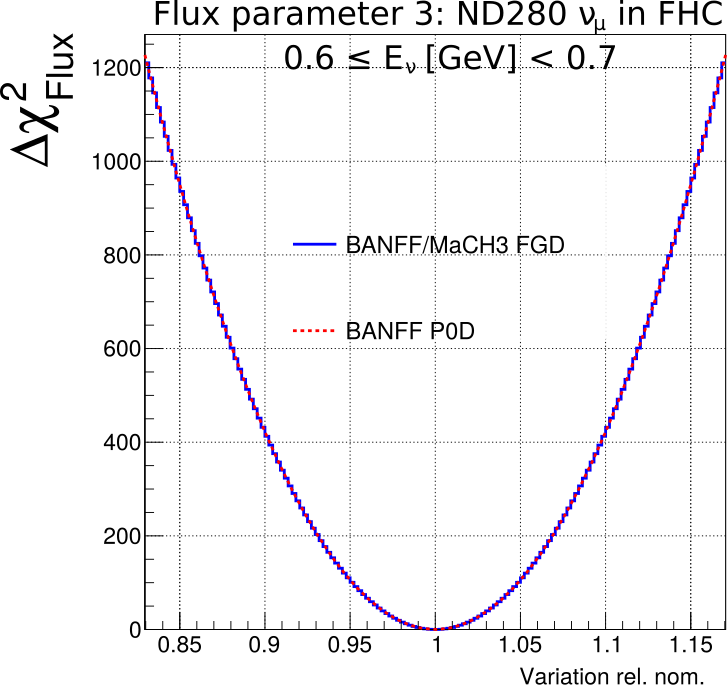
\includegraphics[width=0.45\textwidth]{Chapters/Figures/Validation/Asimov/Flux03Penalty}
\par\end{centering}
}\subfloat[FSI low energy inelastic shape location $\Delta\chi_{\text{xsec}}^{2}$
scan]{\begin{centering}
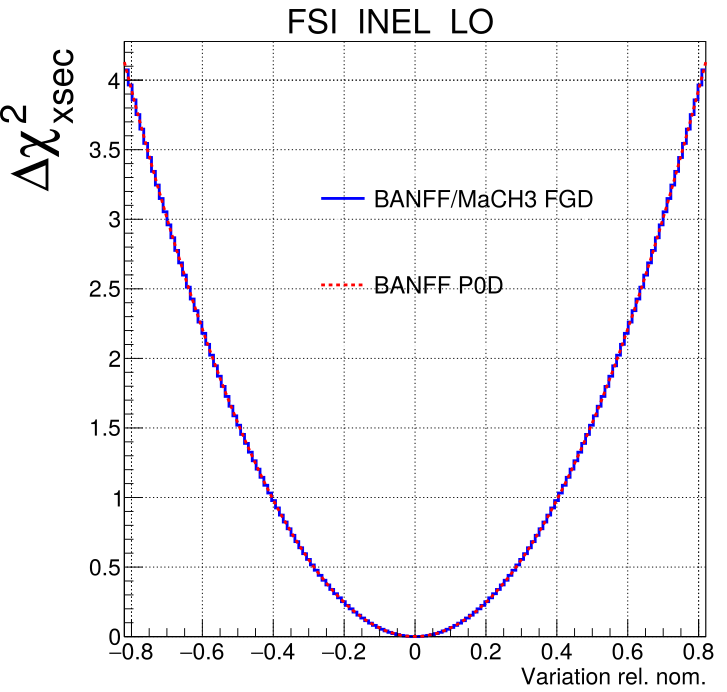
\includegraphics[width=0.45\textwidth]{Chapters/Figures/Validation/Asimov/FSIINELLOPenalty}
\par\end{centering}
}
\par\end{centering}
\caption[Test Statistic Scans for Variations of Fit Parameters in the Asimov
Set]{Comparison of $\Delta\chi^{2}$ scans for variations in fit parameters
in the Asimov set. Two parameters are varied: parameter 3 (left) corresponding
to a flux bin normalization and 562 (right) corresponding to a FSI
shape location parameter. The top panel shows the change in the LLR
test statistic $\Delta\chi_{\text{LLR}}^{2}$ while the bottom panel
shows the penalty terms. In all sub-figures are comparisons between
the BANFF/MaCH3 FGD 2017 results\cite{Abe:2017vif} against the BANFF
$\pod$-only results. Special thanks goes to Clarence Wret (c.wret@rochester.edu)
of the University of Rochester for generating the plots. \label{fig:TestStatisticScans}}
\end{figure}


\subsection{Fit Results}

The postfit results of the Asimov data fit are shown from \prettyref{fig:Asimov-fit-resultsND}
to \prettyref{fig:Asimov-fit-resultsXSEC}. In order to provide a
unified graphical representation for all the parameters, the prefit
and postfit cross section shape parameters are adjusted to be relative
to one (1).

\begin{figure}
\begin{centering}
\subfloat[ND280 $\protect\numu$ in FHC (0-10)]{\begin{centering}
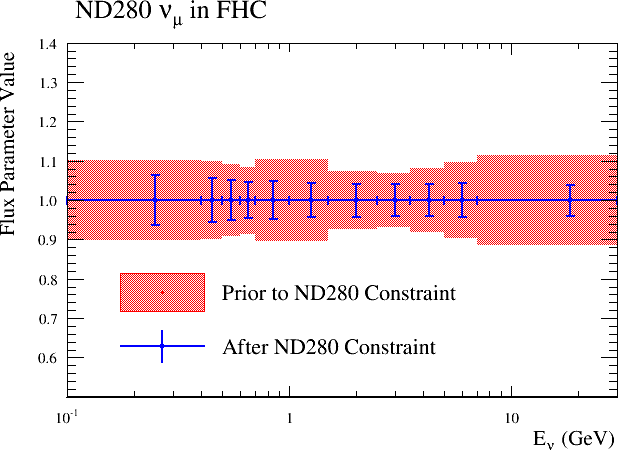
\includegraphics[height=0.195\textheight]{Chapters/Figures/Validation/Asimov/nd_pf_numu_flux_parms}
\par\end{centering}
}\subfloat[ND280 $\protect\numubar$ in FHC (11-15)]{\begin{centering}
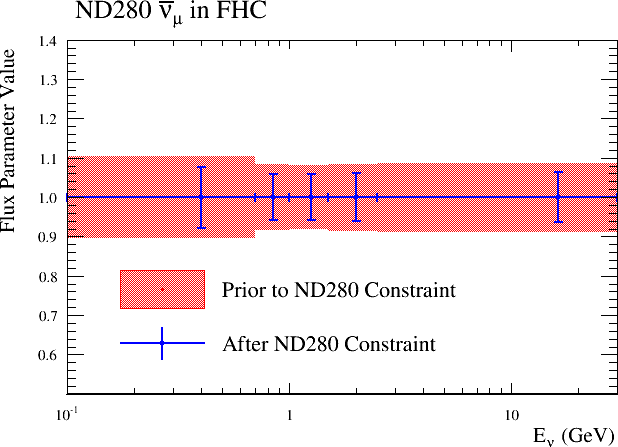
\includegraphics[height=0.195\textheight]{Chapters/Figures/Validation/Asimov/nd_pf_numub_flux_parms}
\par\end{centering}
}
\par\end{centering}
\begin{centering}
\subfloat[ND280 $\protect\nue$ in FHC (16-22)]{\begin{centering}
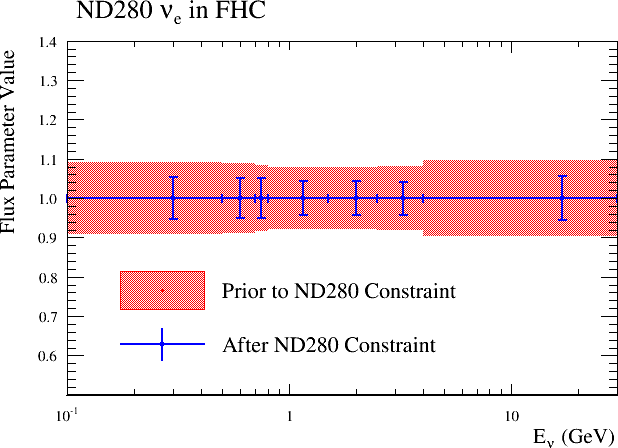
\includegraphics[height=0.195\textheight]{Chapters/Figures/Validation/Asimov/nd_pf_nue_flux_parms}
\par\end{centering}
}\subfloat[ND280 $\protect\nuebar$ in FHC (23-24)]{\begin{centering}
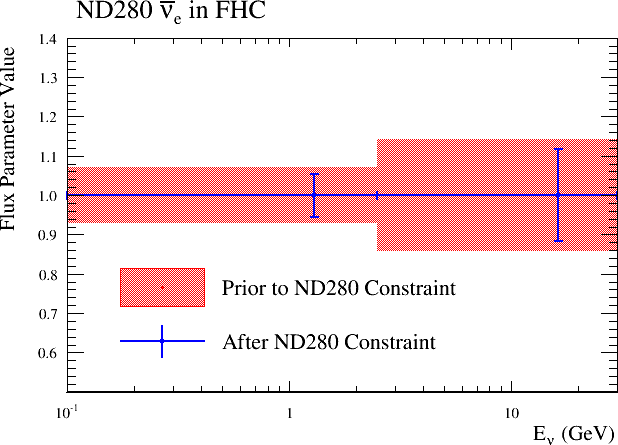
\includegraphics[height=0.195\textheight]{Chapters/Figures/Validation/Asimov/nd_pf_nueb_flux_parms}
\par\end{centering}
}
\par\end{centering}
\begin{centering}
\subfloat[ND280 $\protect\numu$ in RHC (25-29)]{\begin{centering}
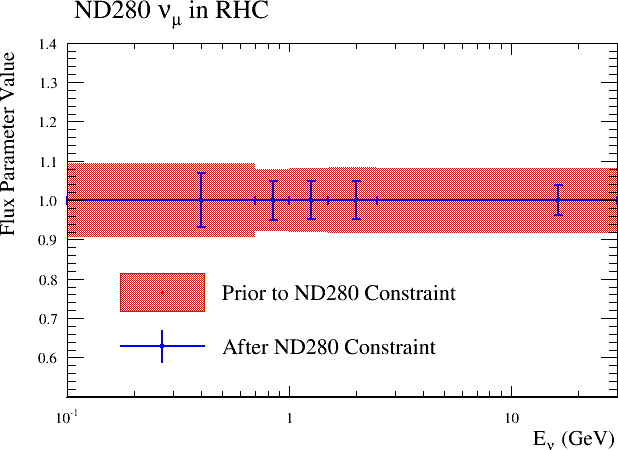
\includegraphics[height=0.195\textheight]{Chapters/Figures/Validation/Asimov/nd_nf_numu_flux_parms}
\par\end{centering}
}\subfloat[ND280 $\protect\numubar$ in RHC (30-40)]{\begin{centering}
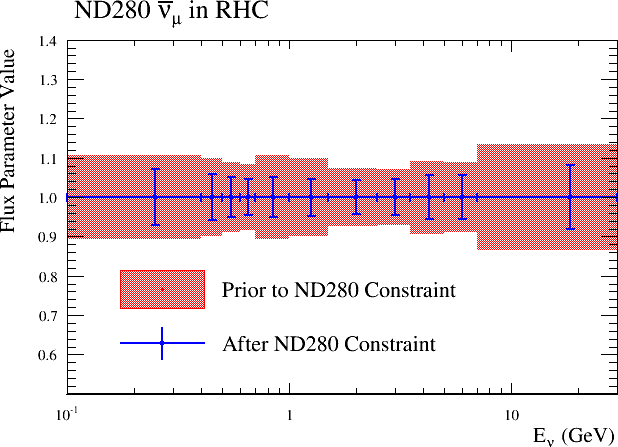
\includegraphics[height=0.195\textheight]{Chapters/Figures/Validation/Asimov/nd_nf_numub_flux_parms}
\par\end{centering}
}
\par\end{centering}
\begin{centering}
\subfloat[ND280 $\protect\nue$ in RHC (41-42)]{\begin{centering}
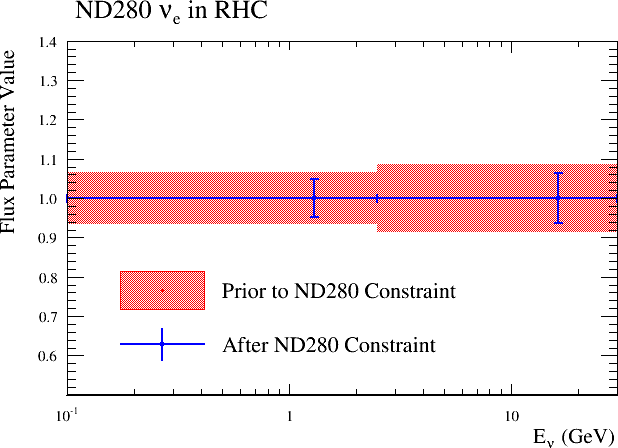
\includegraphics[height=0.195\textheight]{Chapters/Figures/Validation/Asimov/nd_nf_nue_flux_parms}
\par\end{centering}
}\subfloat[ND280 $\protect\nuebar$ in RHC (43-49)]{\begin{centering}
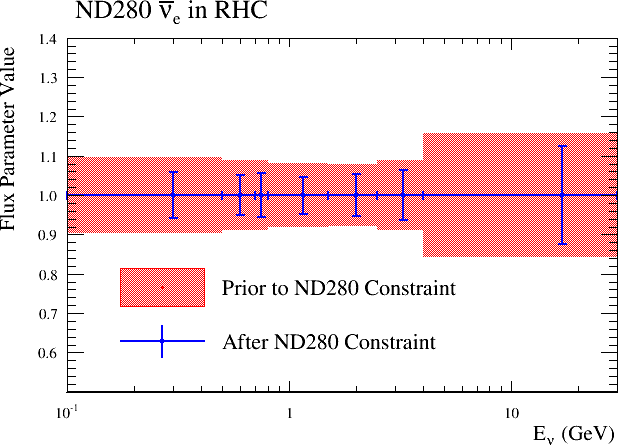
\includegraphics[height=0.195\textheight]{Chapters/Figures/Validation/Asimov/nd_nf_nueb_flux_parms}
\par\end{centering}
}
\par\end{centering}
\caption[Asimov Fit Results for the Flux at ND280]{Asimov fit results for the Flux at ND280. The numbers in parentheses
indicate the fit indices. \label{fig:Asimov-fit-resultsND} }
\end{figure}

\begin{figure}
\begin{centering}
\subfloat[SK $\protect\numu$ in FHC (50-60)]{\begin{centering}
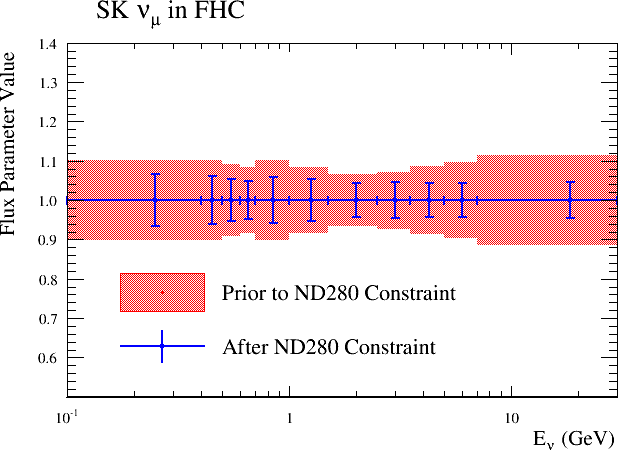
\includegraphics[height=0.195\textheight]{Chapters/Figures/Validation/Asimov/sk_pf_numu_flux_parms}
\par\end{centering}
}\subfloat[SK $\protect\numubar$ in FHC (61-65)]{\begin{centering}
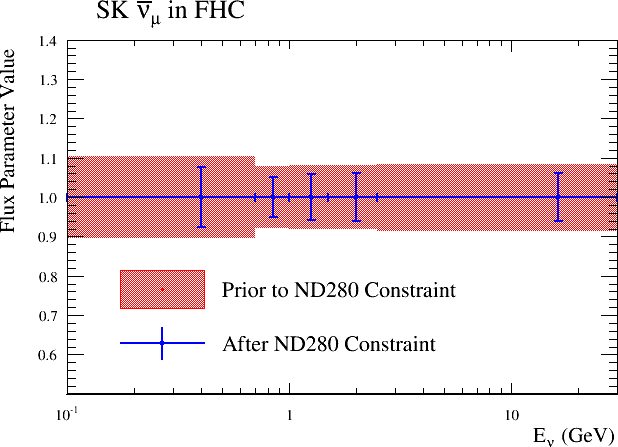
\includegraphics[height=0.195\textheight]{Chapters/Figures/Validation/Asimov/sk_pf_numub_flux_parms}
\par\end{centering}
}
\par\end{centering}
\begin{centering}
\subfloat[SK $\protect\nue$ in FHC (66-72)]{\begin{centering}
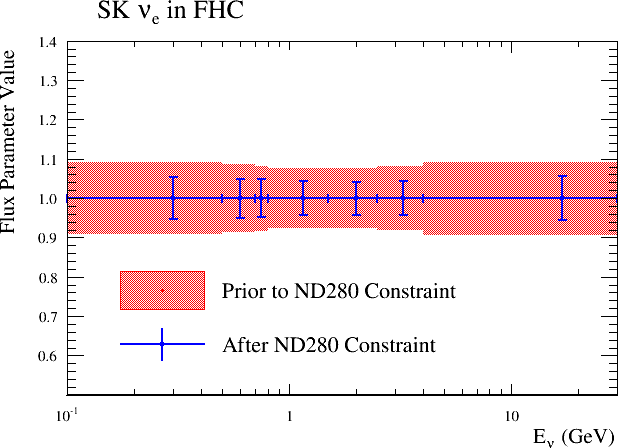
\includegraphics[height=0.195\textheight]{Chapters/Figures/Validation/Asimov/sk_pf_nue_flux_parms}
\par\end{centering}
}\subfloat[SK $\protect\nuebar$ in FHC (73-74)]{\begin{centering}
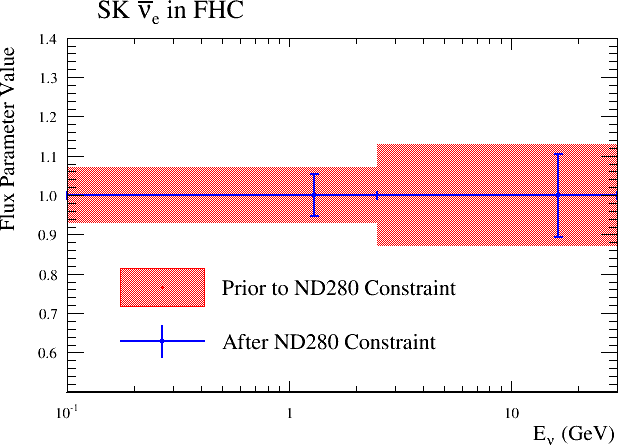
\includegraphics[height=0.195\textheight]{Chapters/Figures/Validation/Asimov/sk_pf_nueb_flux_parms}
\par\end{centering}
}
\par\end{centering}
\begin{centering}
\subfloat[SK $\protect\numu$ in RHC (75-79)]{\begin{centering}
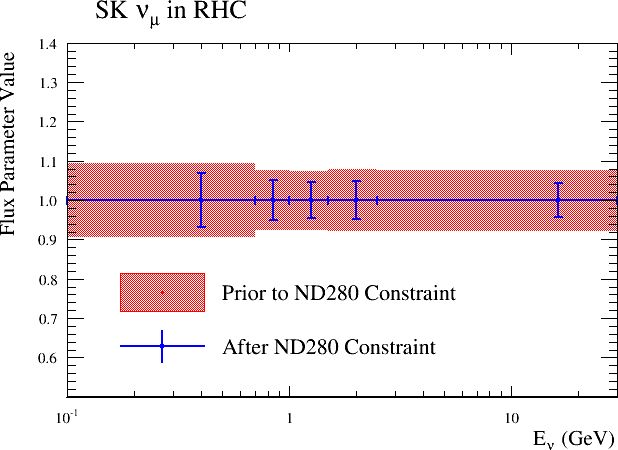
\includegraphics[height=0.195\textheight]{Chapters/Figures/Validation/Asimov/sk_nf_numu_flux_parms}
\par\end{centering}
}\subfloat[SK $\protect\numubar$ in RHC (80-90)]{\begin{centering}
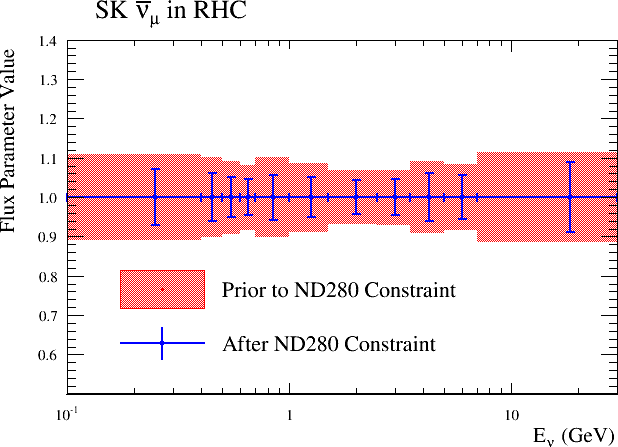
\includegraphics[height=0.195\textheight]{Chapters/Figures/Validation/Asimov/sk_nf_numub_flux_parms}
\par\end{centering}
}
\par\end{centering}
\begin{centering}
\subfloat[SK $\protect\nue$ in RHC (91-92)]{\begin{centering}
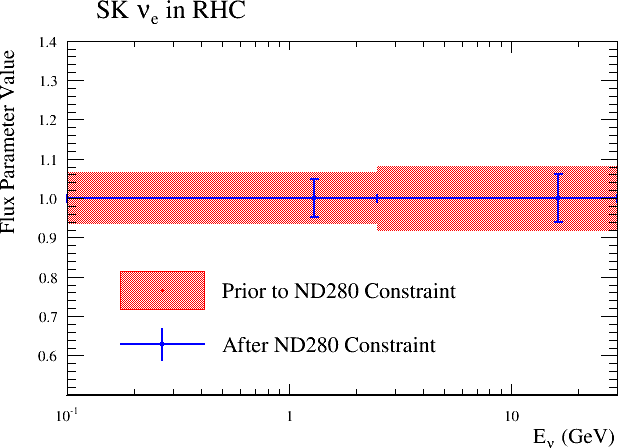
\includegraphics[height=0.195\textheight]{Chapters/Figures/Validation/Asimov/sk_nf_nue_flux_parms}
\par\end{centering}
}\subfloat[SK $\protect\nuebar$ in RHC (93-99)]{\begin{centering}
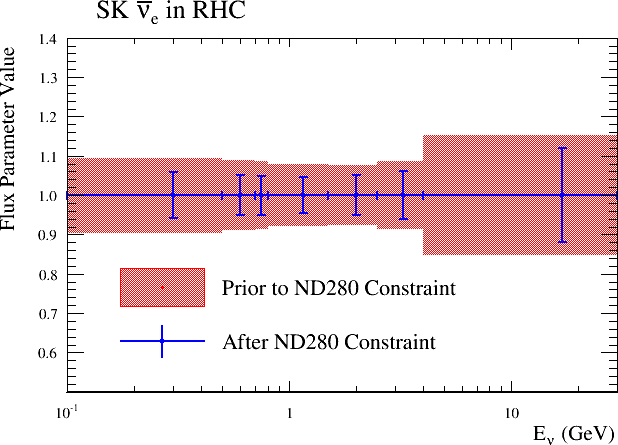
\includegraphics[height=0.195\textheight]{Chapters/Figures/Validation/Asimov/sk_nf_nueb_flux_parms}
\par\end{centering}
}
\par\end{centering}
\caption[Asimov Fit Results for the Flux at Super-K]{Asimov fit results for the Flux at Super-K. The numbers in parentheses
indicate the fit indices . \label{fig:Asimov-fit-resultsSKFHC} }
\end{figure}

\begin{figure}
\begin{centering}
\subfloat[Water-in obsnorms (100 - 330)]{\begin{centering}
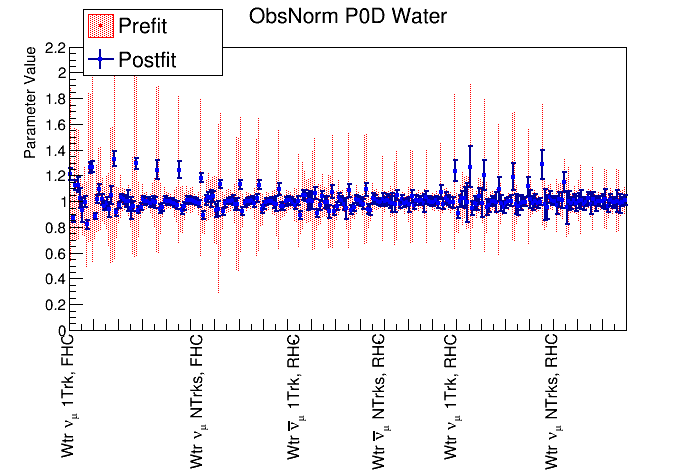
\includegraphics[height=0.4\textheight]{Chapters/Figures/Validation/Asimov/ParameterPlots_ObsNorm_P0D_Water}
\par\end{centering}
}
\par\end{centering}
\begin{centering}
\subfloat[Water-out obsnorms (331-561)]{\begin{centering}
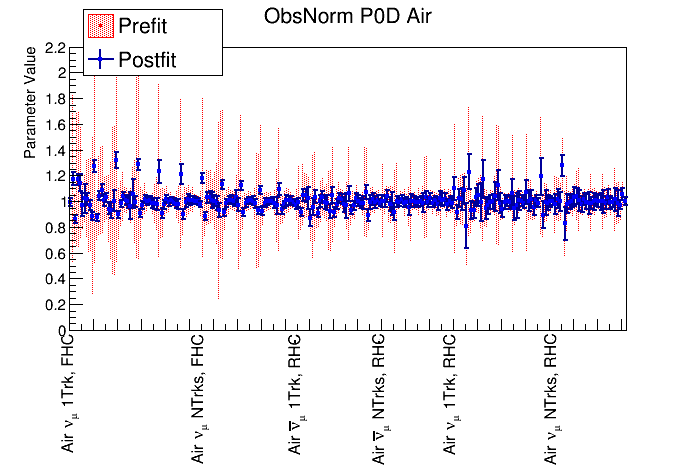
\includegraphics[height=0.4\textheight]{Chapters/Figures/Validation/Asimov/ParameterPlots_ObsNorm_P0D_Air}
\par\end{centering}
}
\par\end{centering}
\caption[Asimov Fit Results for the Bin Normalization Parameters]{Asimov fit results for the obsnorm parameters. The numbers in parentheses
indicate the fit indices. The large jumps in the bin normalization
parameters is an artifact of the indexing choice with the indices
increasing in increasing momentum in constant angular slices. Compare
the changes in the bin normalizations in the $\protect\numu$ in FHC
Mode CC 1-Track in \prettyref{fig:Bin-normalization-edgesNumuFHC}.
\label{fig:Asimov-fit-resultsObsnorm}}
\end{figure}

\begin{figure}
\begin{centering}
\subfloat[FSI (562-567)]{\begin{centering}
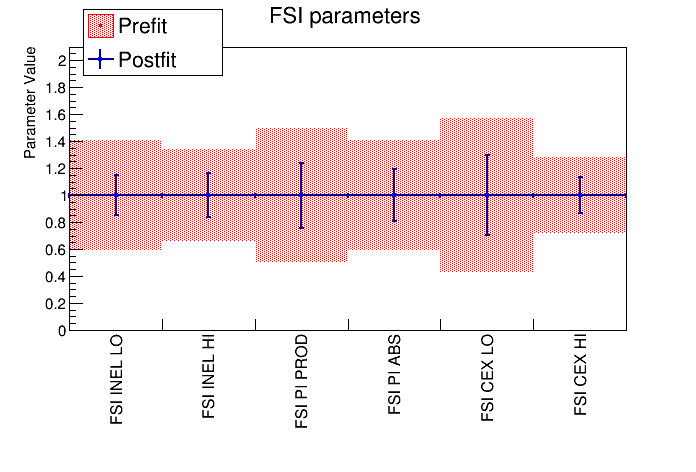
\includegraphics[height=0.4\textheight]{Chapters/Figures/Validation/Asimov/FSI_parameters}
\par\end{centering}
}
\par\end{centering}
\begin{centering}
\subfloat[Cross Section (568-592)]{\begin{centering}
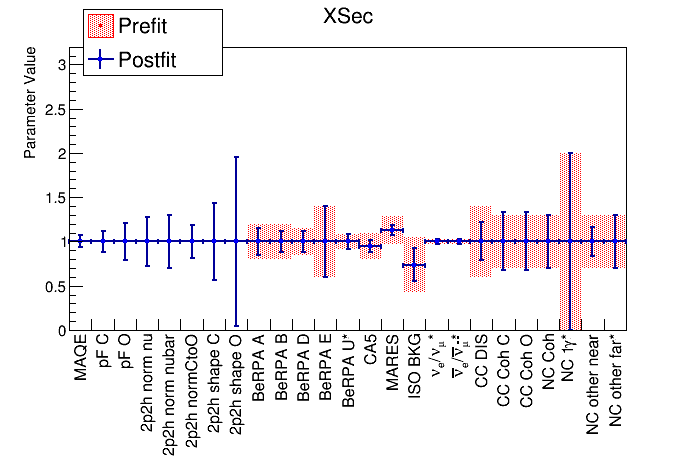
\includegraphics[height=0.4\textheight]{Chapters/Figures/Validation/Asimov/ParameterPlots_XSec}
\par\end{centering}
}
\par\end{centering}
\caption[Asimov Fit Results for the Cross Section and FSI Parameters]{Asimov fit results for the FSI and cross section parameters. The numbers
in parentheses indicate the fit indices. In order to provide a consistent
presentation of parameter changes between prefit and postfit among
all parameters, shape location and scale parameters are adjusted to
prefits of one (1). In effect, the value and uncertainties for all
parameters are fractional changes. \label{fig:Asimov-fit-resultsXSEC}}
\end{figure}

We see that the postfit parameters have uncertainties that are different
compared to their prefit values. This is expected since correlations
between the sub-matrices in the covariance matrix, which were assumed
uncorrelated to start, have been calculated. The complete postfit
correlation matrix is shown in \prettyref{fig:Complete-postfit-correlation}
and the flux and cross section only correlation matrix is shown in
\prettyref{fig:XsecFlux-postfit-correlation}. We observe significant
anti-correlations between each of the sub-matrices, which is predicted
from \eqref{eq:n-predicted-general} since any increase in one parameter
weight forces a decrease in the others.

\begin{figure}
\begin{centering}
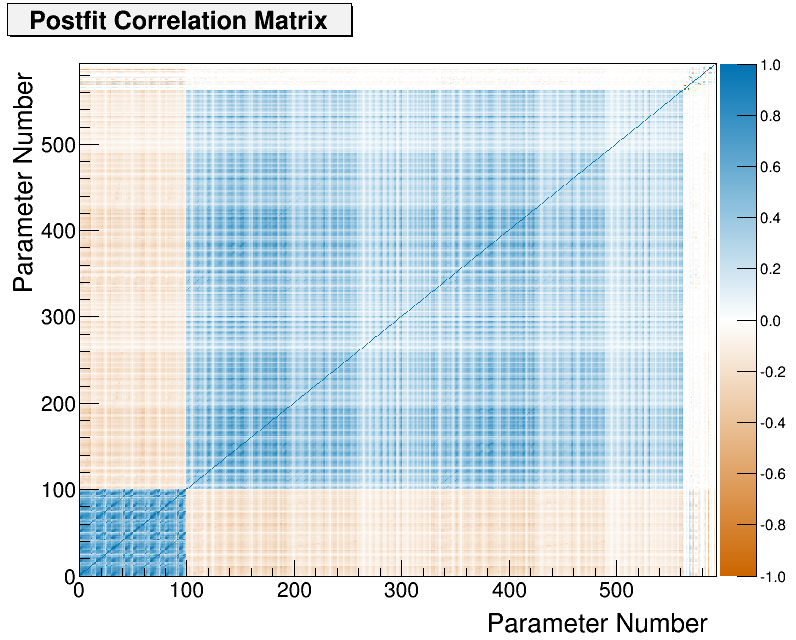
\includegraphics[height=0.4\textheight]{Chapters/Figures/Validation/Asimov/corr_post}
\par\end{centering}
\caption[Complete Postfit Correlation Matrix for the Asimov Data Fit]{Complete postfit correlation matrix for the Asimov data fit.\label{fig:Complete-postfit-correlation}}
\end{figure}

\begin{figure}
\begin{centering}
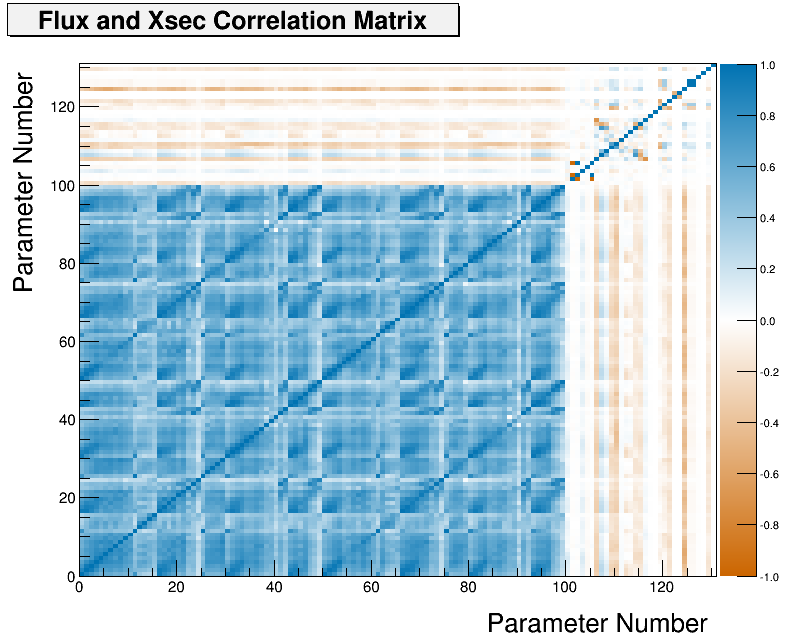
\includegraphics[height=0.4\textheight]{Chapters/Figures/Validation/Asimov/corr_flux_xsec}
\par\end{centering}
\caption[Flux and Cross Section Postfit Correlation Matrix for the Asimov Data
Fit]{Flux and cross section postfit correlation matrix for the Asimov data
fit. The parameters from 1-100 are the flux parameters and all parameters
after are the cross section. \label{fig:XsecFlux-postfit-correlation}}
\end{figure}


\section{Fake Data Fits\label{sec:Fake-Data-Fits}}

In this section, we examine the results of BANFF fits when given data
sets with nonphysical alterations. As stated earlier, these are called
fake data sets since we are treating these as data in the fit. The
fake data sets initially start as the Asimov data set and have variations
applied to them. Here we are only interested in varying the flux and
cross section parameters since they are the parameters that are propagated
to the oscillation analysis. There were two fake data sets generated
for the tests. One data set varies the neutrino flux in a single flux
bin and the other varies the single pion production rate.

While other fake data sets could be generated that are more or less
similar to the Asimov data set, that is not the purpose of fitting
to fake data sets. \textit{The purpose of these tests is to show the
fit can converge when provided with non-Asimov data sets and we can
understand the results.} It is known in the BANFF group that the BANFF
fitting software is not guaranteed to converge on a global minimum
when using altered Asimov data. In particular, fitting FGD-only data
generated from random and uncorrelated variations of all fit flux,
cross section, and bin normalization parameters, 127 out of 500 fits
(\textasciitilde 25\%) reported fit convergence problems. So convergence
is not assured in all situations, but is possible. We can establish
that a credible $\pod$-only real data fit result is possible by demonstrating
1) the BANFF fit converges with $\pod$-only fake data and 2) that
we can sensibly understand those fit results.

The information provided from fake data tests is also useful to understand
possible biases in the fit results. For instance, since the $\pod$
samples have a relatively low sensitivity to CC-$1\pi$ interactions,
real differences between data and MC could be explained by variations
in non CC-$1\pi$ model parameters. We will get a sense of the biases
in the following two fake data tests. The first fake data test analyzed
is referred to as the ``High Energy Neutrino Flux Variation'' which
varies the high energy $\numu$ flux in FHC mode. The following fake
data test is referred to as the ``Single Pion Event Rate Variation''
which alters the single pion production event rate uniformly.

\subsection{High Energy Neutrino Flux Variation}

This fake data set is almost identical to the Asimov data set expect
an arbitrarily large increase in the $\numu$ flux between 7 and 30
GeV by +25\% in FHC mode only. This variation was chosen since this
energy range corresponds precisely to flux parameter $b_{10}$ and
it could affect all analysis bins. The true neutrino energy distribution
of the fake data used in this study is shown in \prettyref{fig:Neutrino-flux-fake-data-set}
and \prettyref{fig:Neutrino-flux-fake-data-set-1}.

\begin{figure}
\begin{centering}
\subfloat[The $\protect\numu$ in FHC Mode CC 1-Track sample]{\begin{centering}
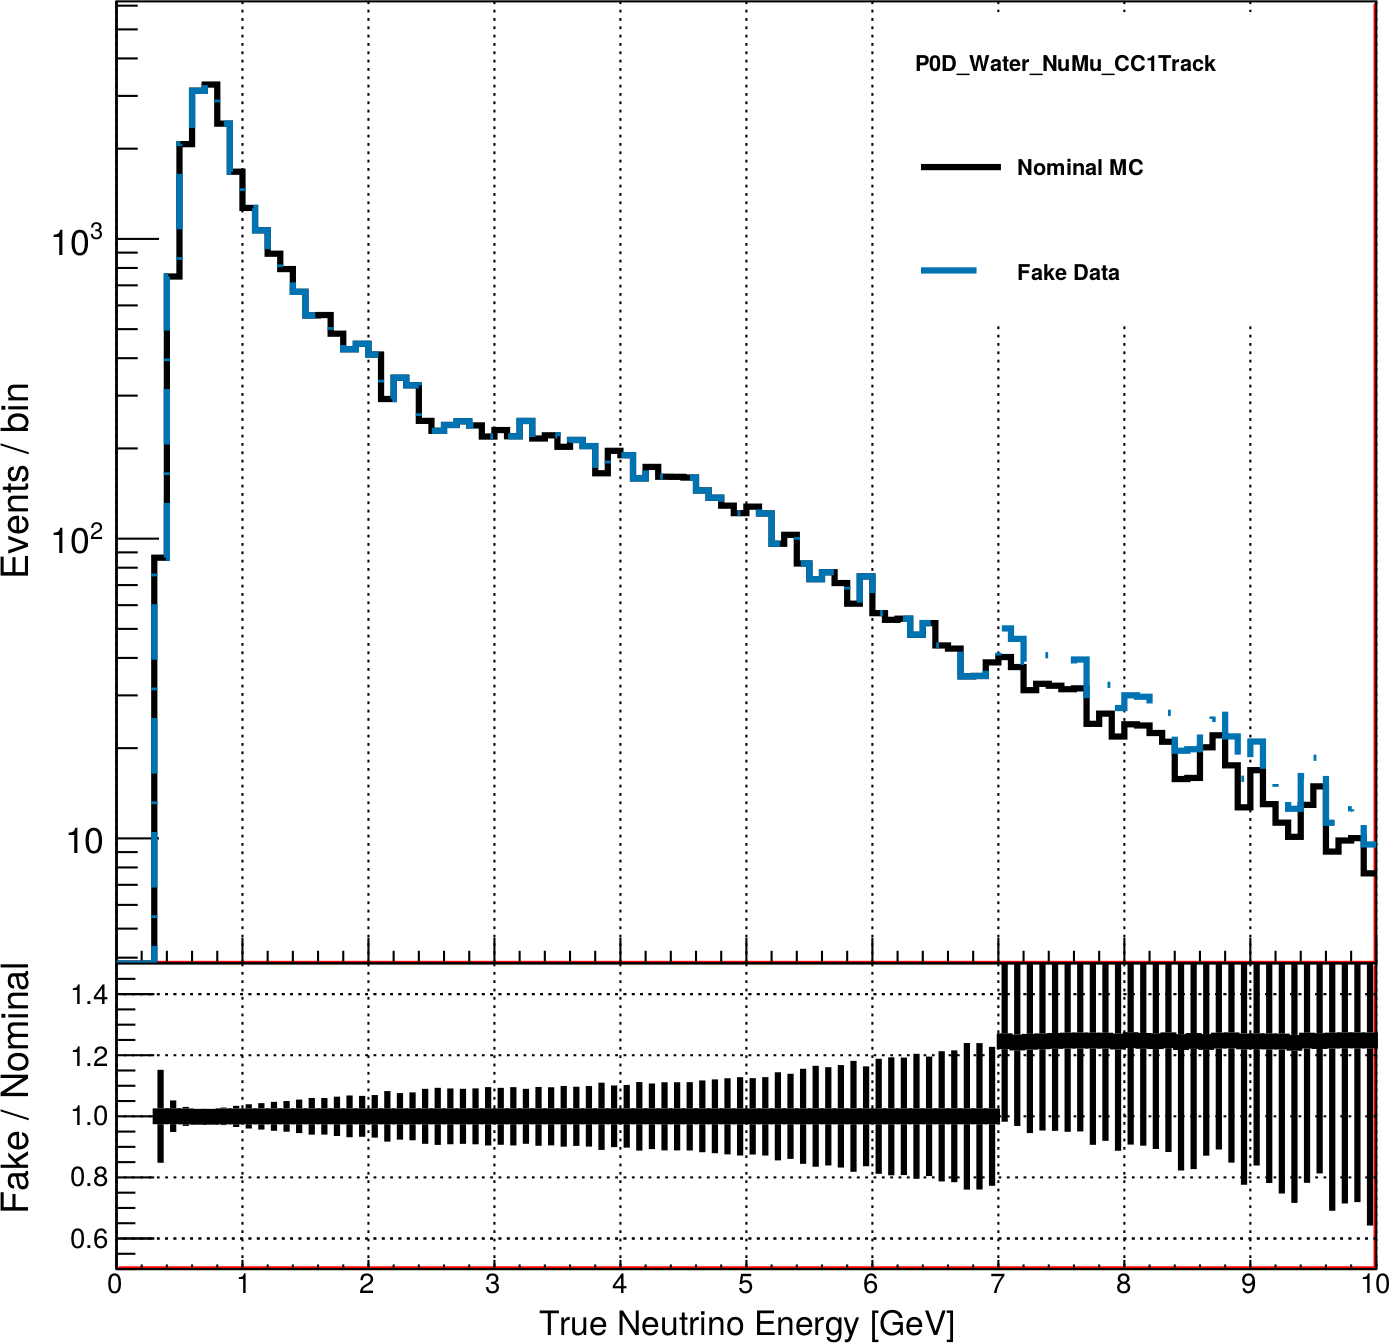
\includegraphics[height=0.4\textheight]{Chapters/Figures/Validation/NuMuFluxVariationFakeData/NuMu1Trk}
\par\end{centering}
}
\par\end{centering}
\begin{centering}
\subfloat[The $\protect\numu$ in FHC Mode CC N-Tracks sample]{\begin{centering}
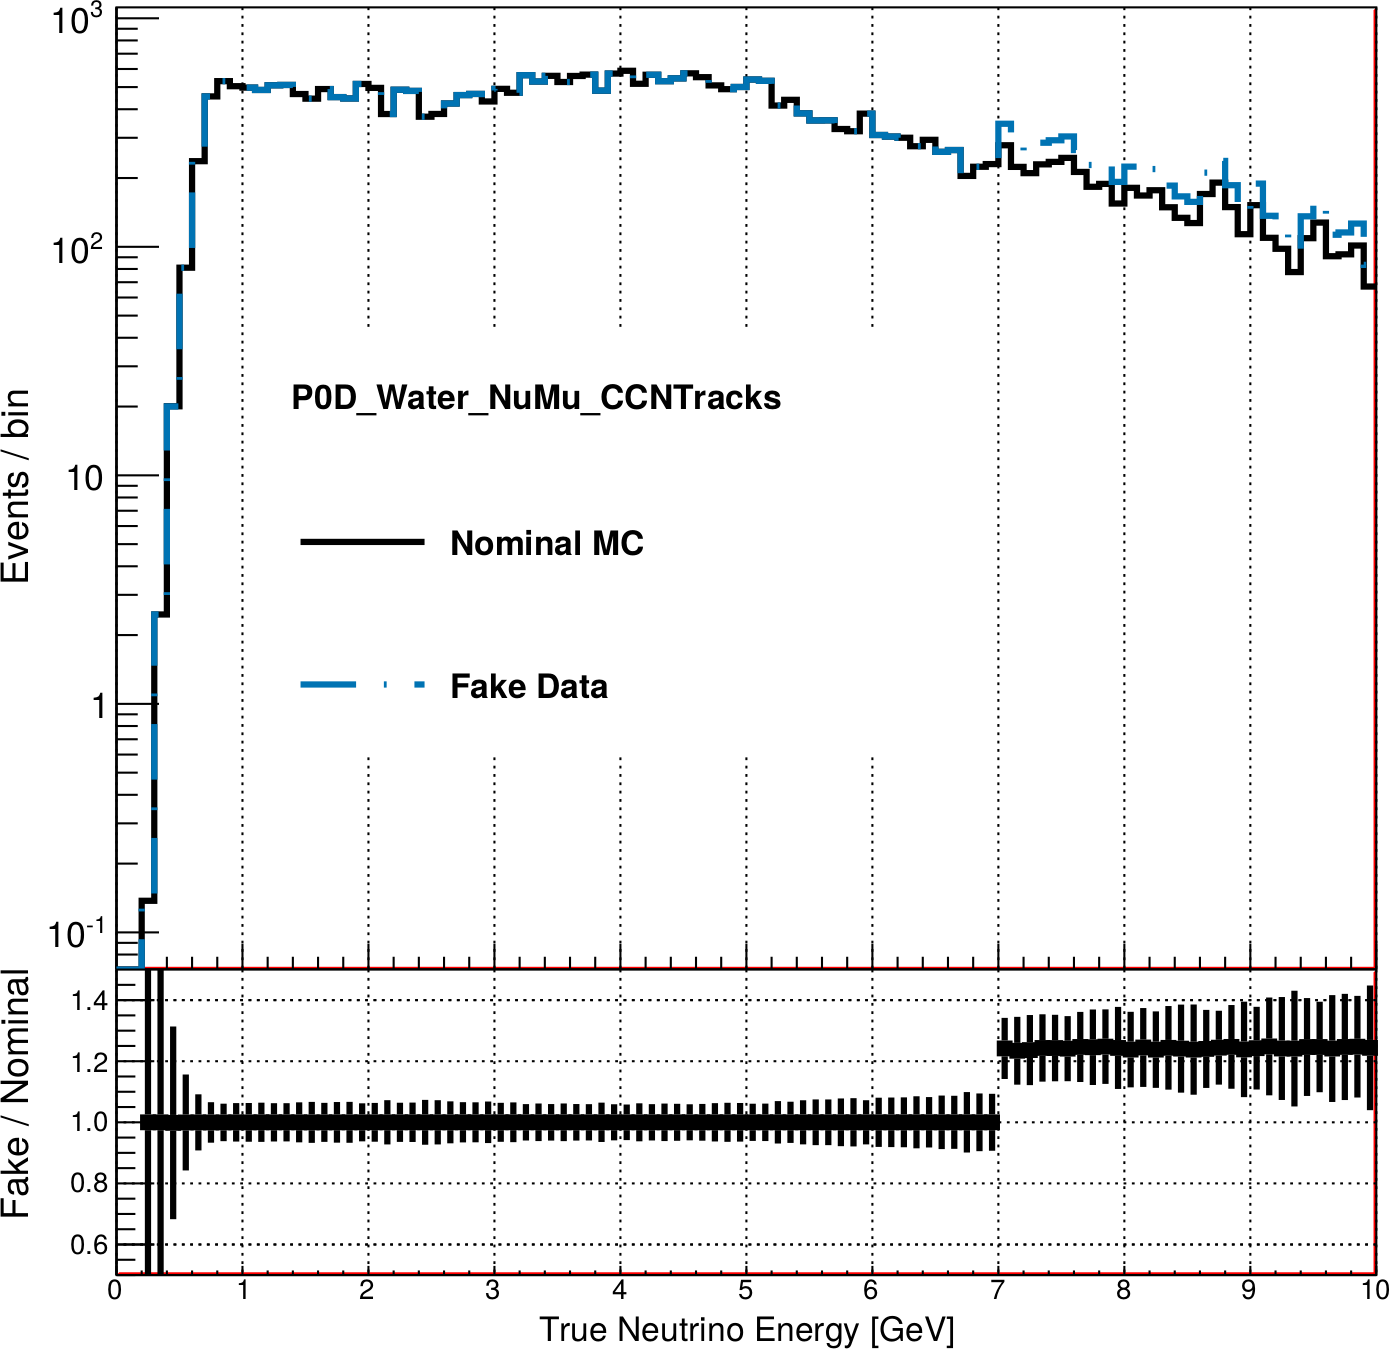
\includegraphics[height=0.4\textheight]{Chapters/Figures/Validation/NuMuFluxVariationFakeData/NuMuNTrks}
\par\end{centering}
}
\par\end{centering}
\caption[Neutrino Energy Distributions in the High Energy Neutrino Flux Variation
Fake Data Set]{Neutrino energy distributions in the High Energy Neutrino Flux variation
fake data set. The fake data (dashed-blue) is nearly identical to
the Asimov set (black) except the +25\% increase in the $\protect\numu$
in FHC mode rate at energies greater than 7 GeV. In the figures, ``Nominal
MC'' refers to the Asimov prediction and ``Fake Data'' is the altered
data set. The ratio of the fake data to the nominal MC is shown below
each histogram with the errors being statistical only.\label{fig:Neutrino-flux-fake-data-set}}
\end{figure}
\begin{figure}
\begin{centering}
\subfloat[The $\protect\numubar$ in RHC Mode CC 1-Track sample]{\begin{centering}
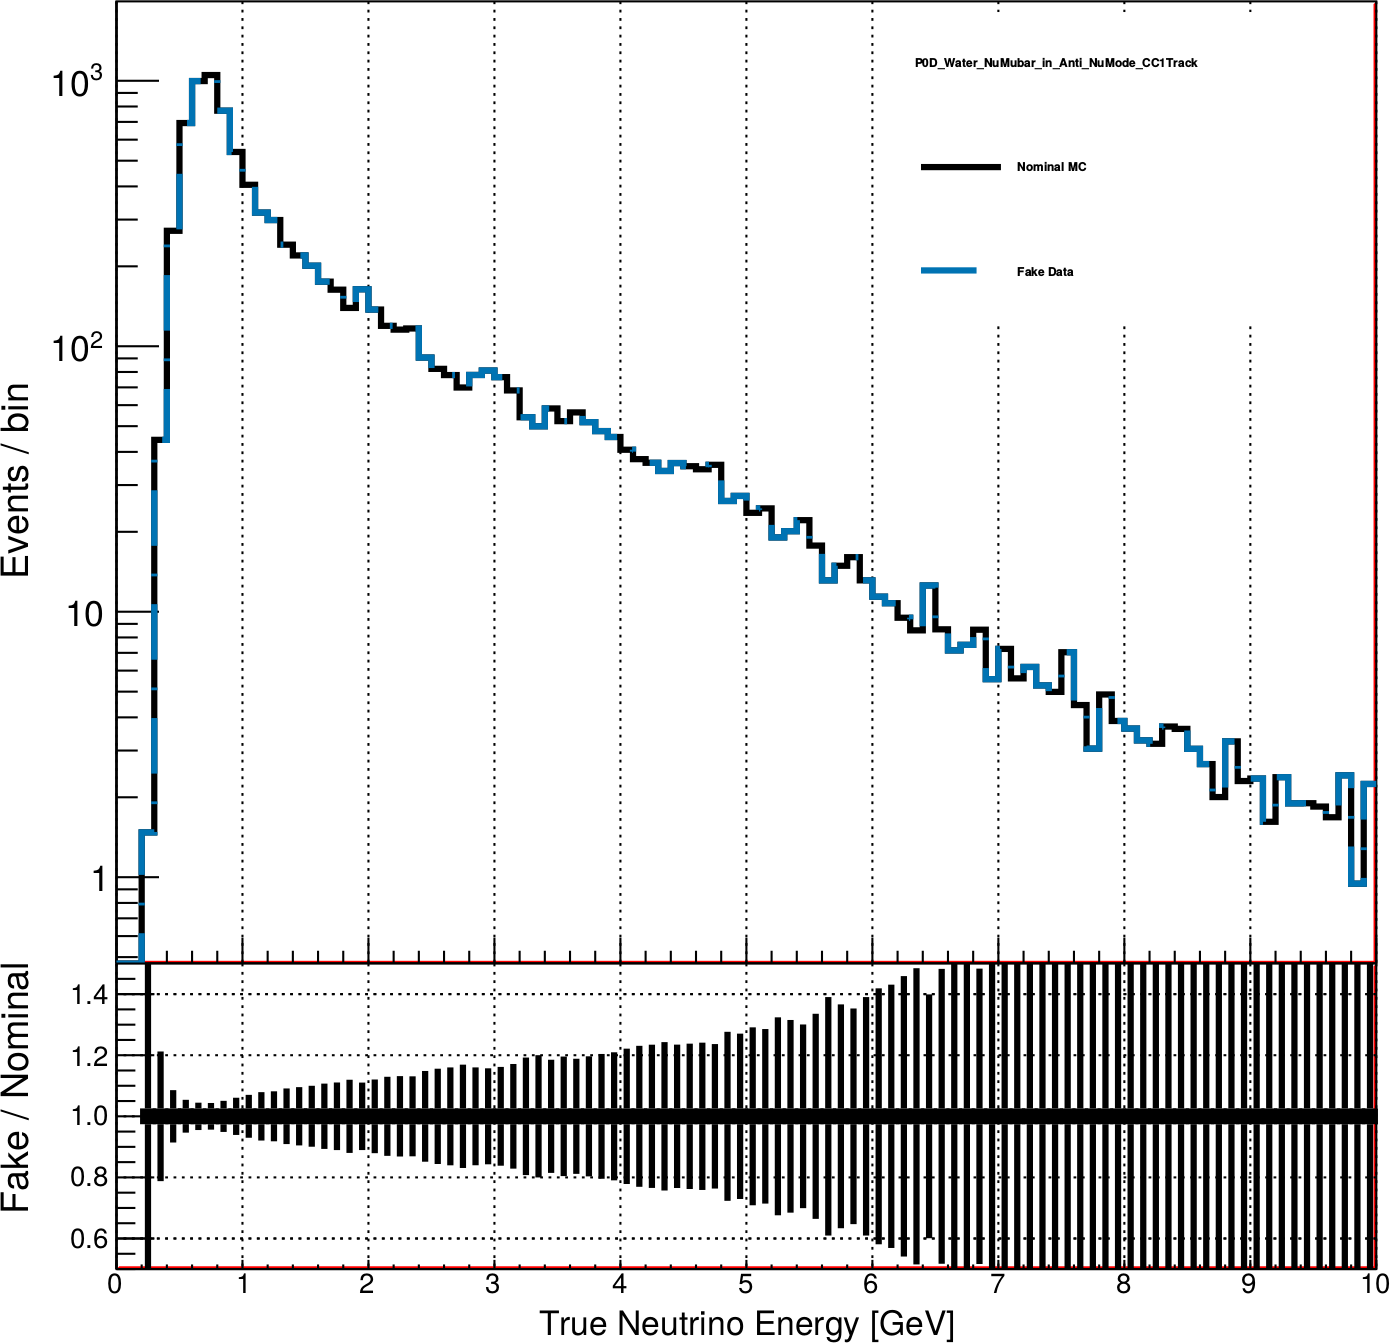
\includegraphics[width=0.48\textwidth]{Chapters/Figures/Validation/NuMuFluxVariationFakeData/ANuMuRHC1Trk}
\par\end{centering}
}\subfloat[The $\protect\numubar$ in RHC Mode CC N-Tracks sample]{\begin{centering}
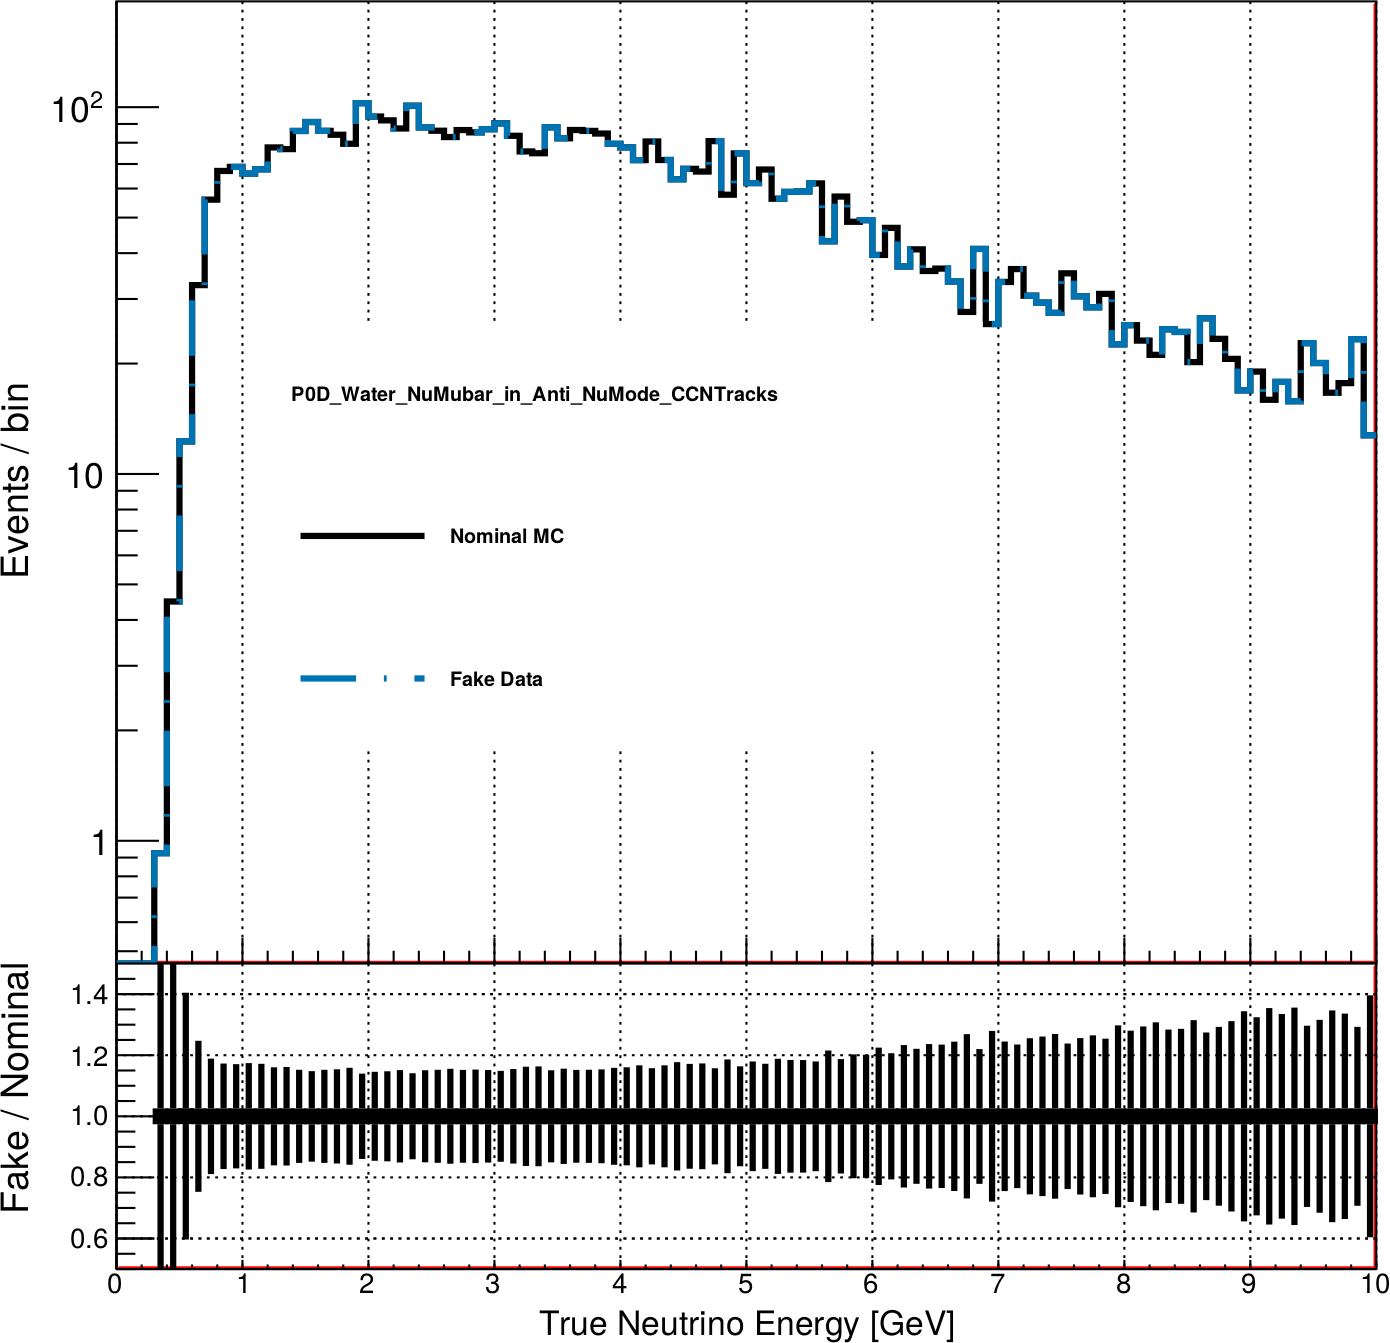
\includegraphics[width=0.48\textwidth]{Chapters/Figures/Validation/NuMuFluxVariationFakeData/ANuMuRHCNTrks}
\par\end{centering}
}
\par\end{centering}
\begin{centering}
\subfloat[The $\protect\numu$ in RHC Mode CC 1-Track sample]{\begin{centering}
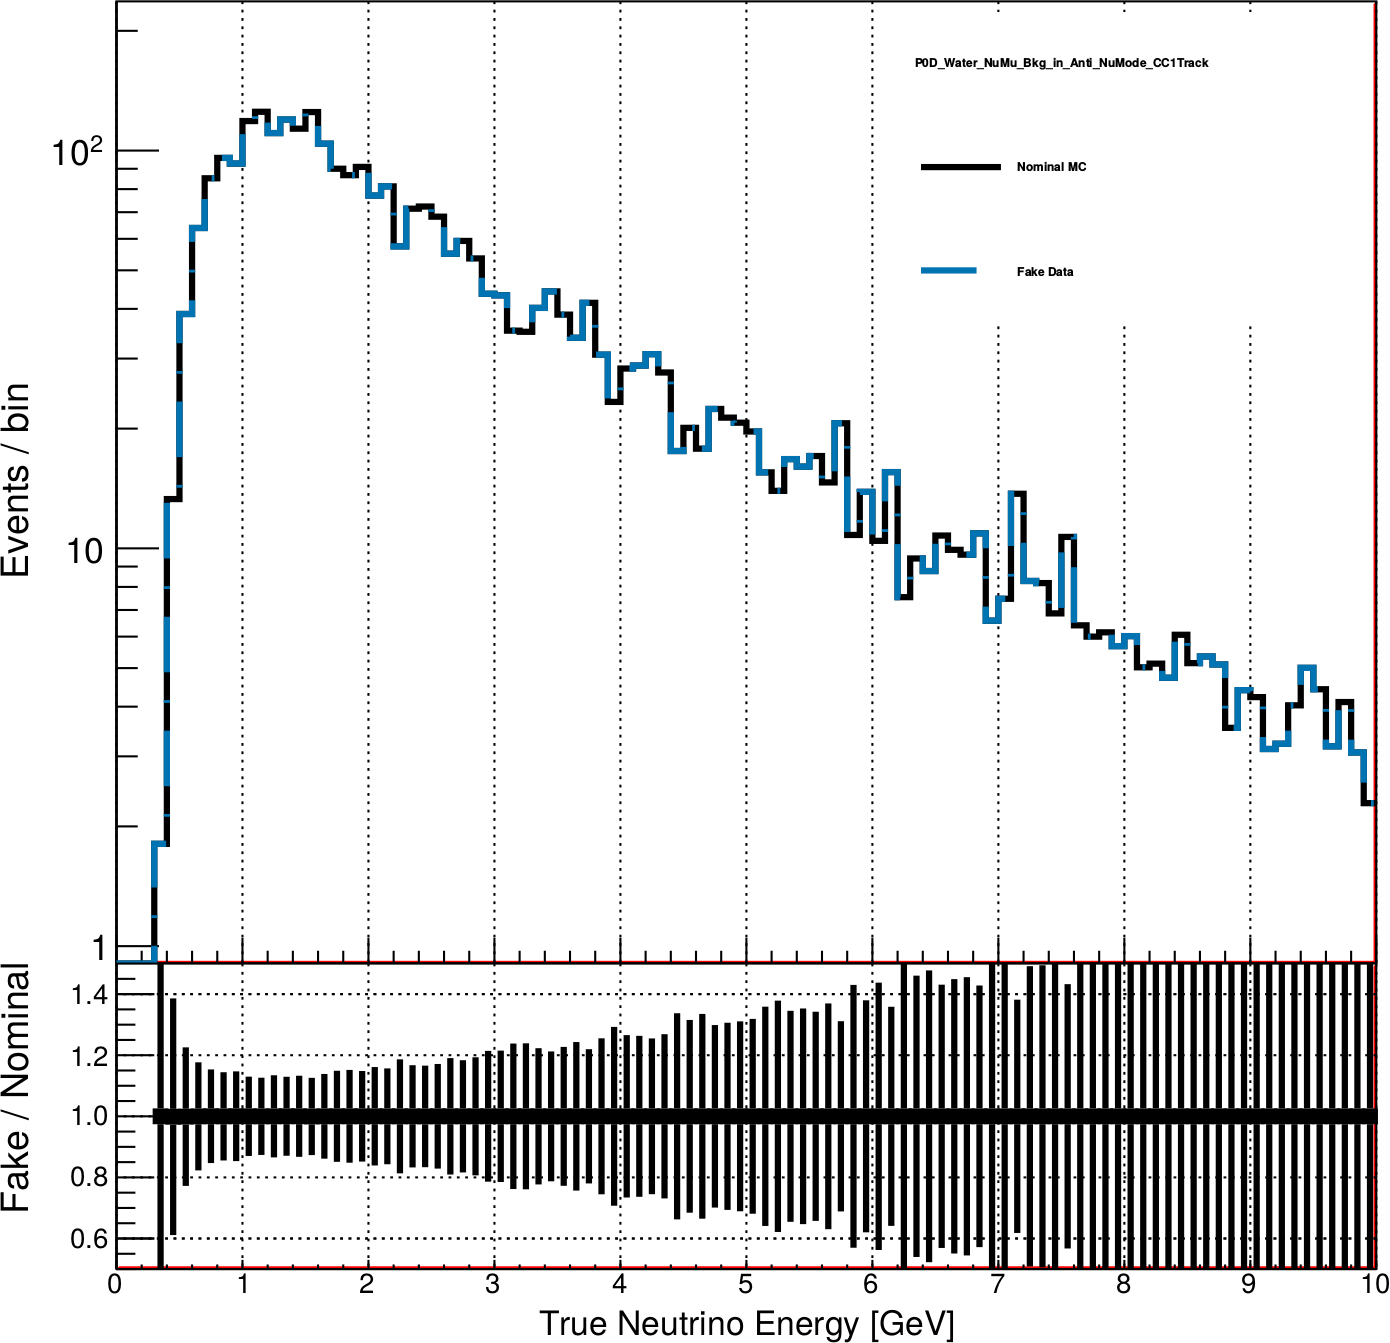
\includegraphics[width=0.48\textwidth]{Chapters/Figures/Validation/NuMuFluxVariationFakeData/NuMuRHC1Trk}
\par\end{centering}
}\subfloat[The $\protect\numu$ in RHC Mode CC N-Tracks sample]{\begin{centering}
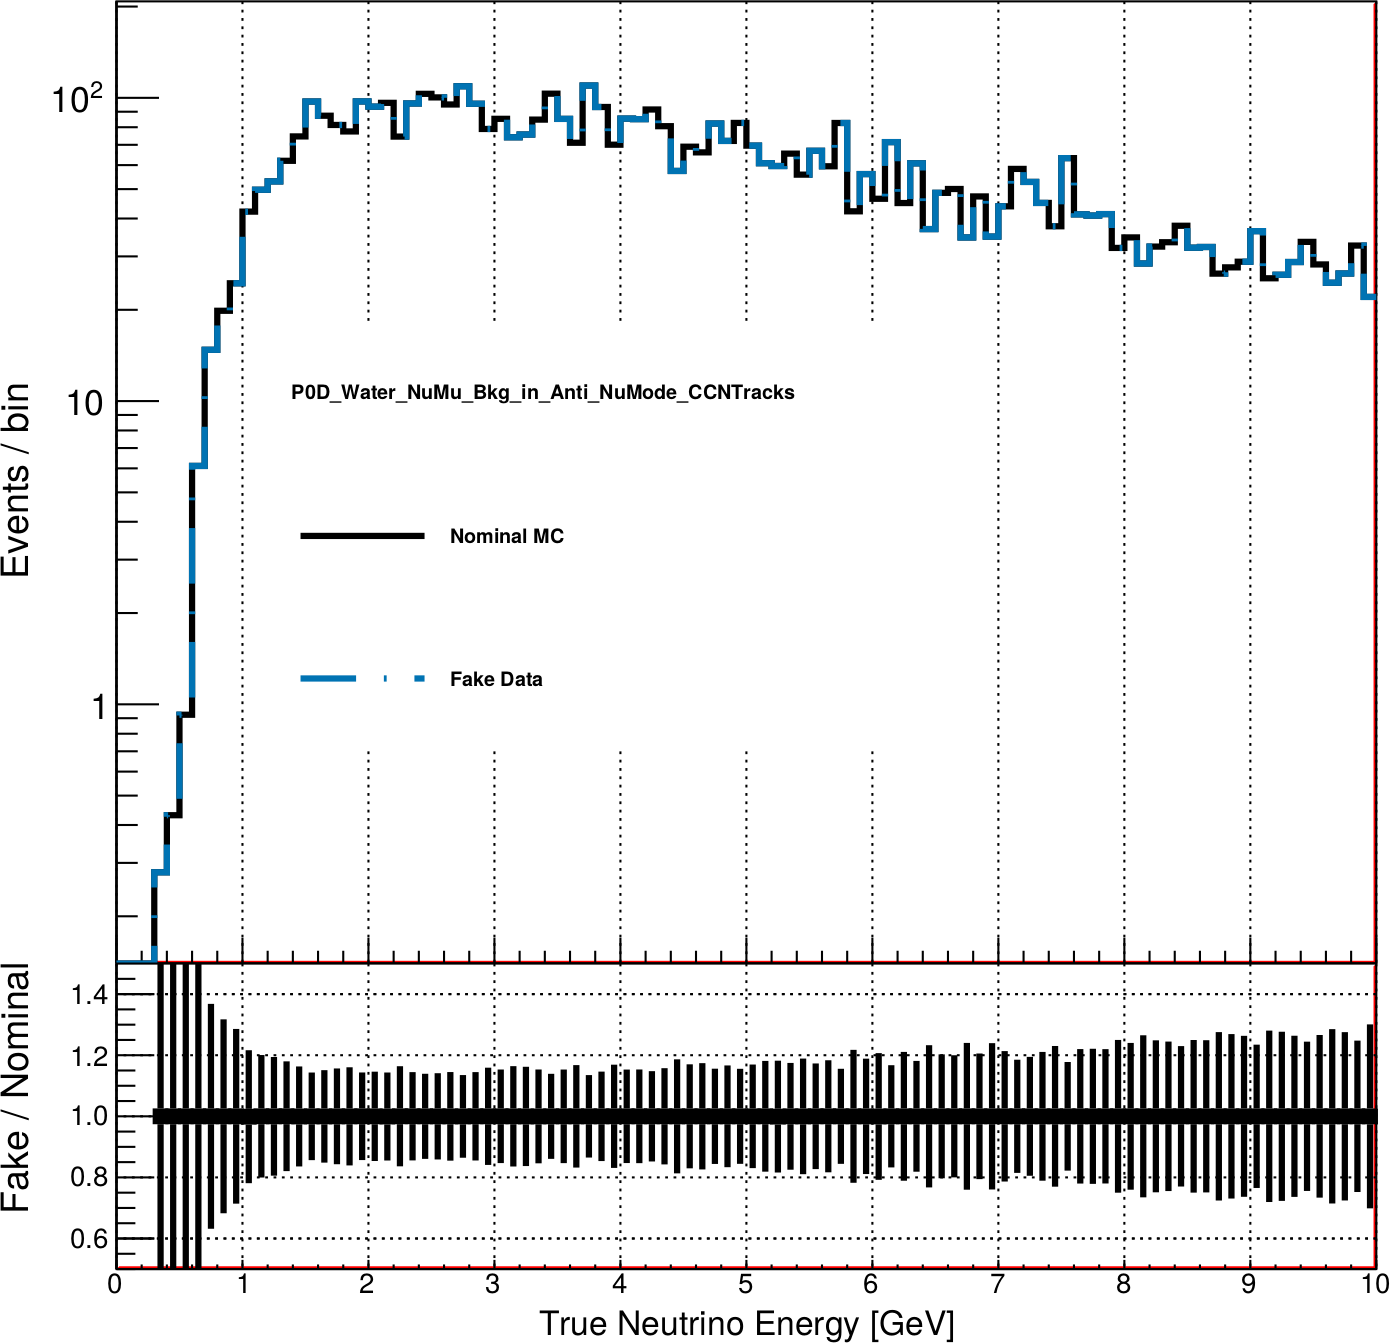
\includegraphics[width=0.48\textwidth]{Chapters/Figures/Validation/NuMuFluxVariationFakeData/NuMuRHCNTrks}
\par\end{centering}
}
\par\end{centering}
\caption[Neutrino Energy Distributions in the High Energy Neutrino Flux Variation
Fake Data Set (Continued)]{Neutrino energy distributions in the High Energy Neutrino Flux variation
fake data set (continued). The fake data (dashed-blue) is nearly identical
to the Asimov set (black) except the +25\% increase in the $\protect\numu$
in FHC mode rate at energies greater than 7 GeV. In the figures, ``Nominal
MC'' refers to the Asimov prediction and ``Fake Data'' is the altered
data set. The ratio of the fake data to the nominal MC is shown below
each histogram with the errors being statistical only.\label{fig:Neutrino-flux-fake-data-set-1}}
\end{figure}

The postfit parameter plots are shown in \prettyref{fig:Postfit-numu-flux-fake-data}.
We see that the target flux parameter $b_{10}$ has significantly
increased from its prefit value by almost +20\%. However, due to correlations
in the flux covariance matrix, other flux parameters have also changed.
The BANFF fit prefers to increase the previous energy flux parameter
and the high energy $\nue$ flux parameters as well. While we saw
that the flux and hence event rate was not changed in the RHC samples,
the RHC flux parameters are also slightly affected. However, the RHC
flux parameters are still well within prefit uncertainties. The statement
is true for the cross section and FSI parameters. We can conclude
from this study that the fit will resolve large, nonphysical differences
between the Asimov prediction and the data with many correlated parameter
variations.

\begin{figure}
\begin{centering}
\subfloat[The ND280 FHC mode flux parameters]{\begin{centering}
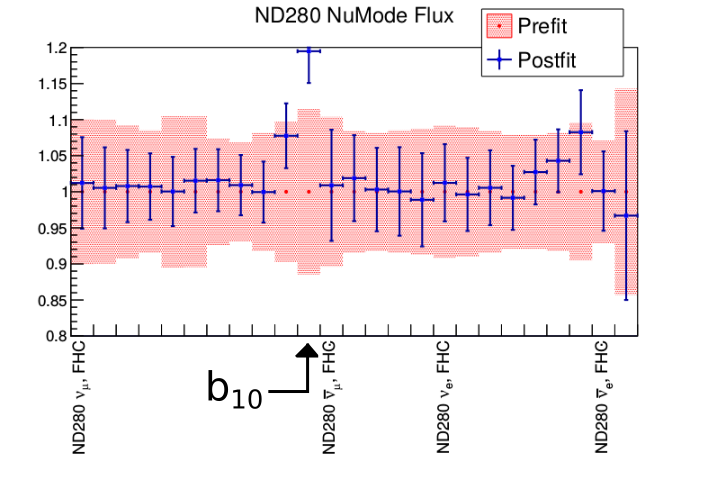
\includegraphics[width=0.48\textwidth]{Chapters/Figures/Validation/NuMuFluxVariationFakeData/ND280NuMu_b10Shown}
\par\end{centering}
}\subfloat[The ND280 RHC mode flux parameters]{\begin{centering}
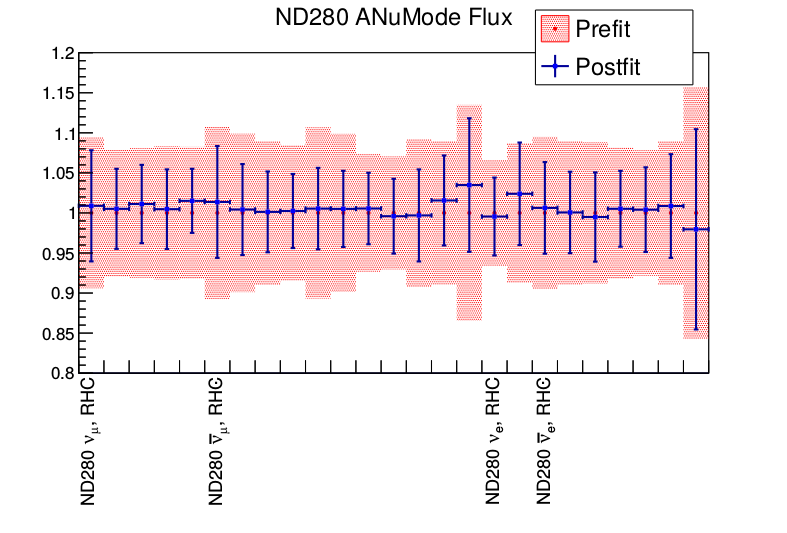
\includegraphics[width=0.48\textwidth]{Chapters/Figures/Validation/NuMuFluxVariationFakeData/ND280ANuMu}
\par\end{centering}
}
\par\end{centering}
\begin{centering}
\subfloat[Cross section parameters]{\begin{centering}
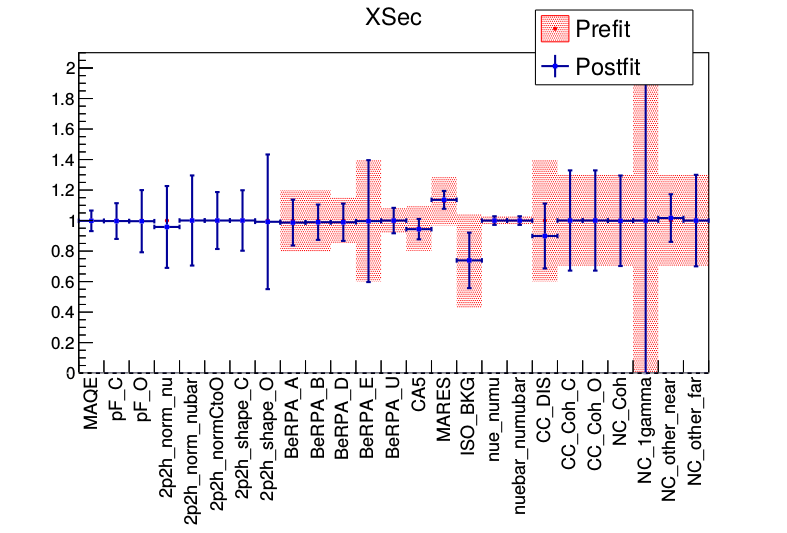
\includegraphics[width=0.48\textwidth]{Chapters/Figures/Validation/NuMuFluxVariationFakeData/XSec}
\par\end{centering}
}\subfloat[The FSI parameters]{\begin{centering}
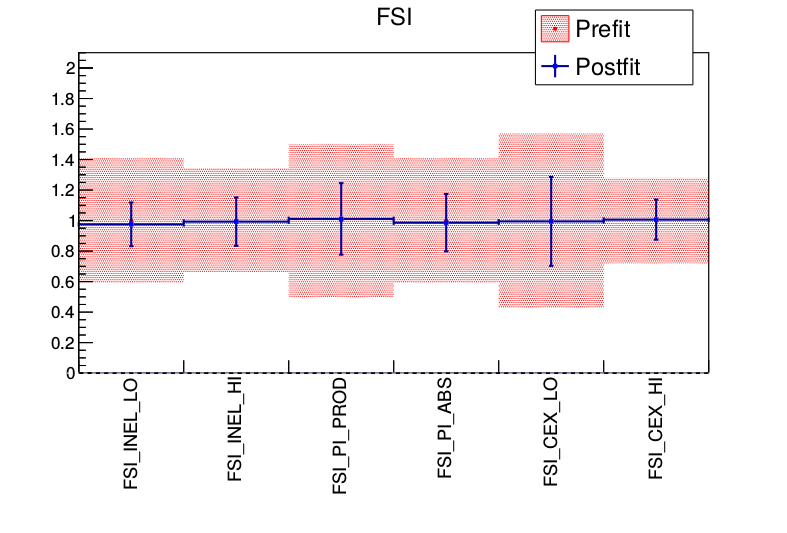
\includegraphics[width=0.48\textwidth]{Chapters/Figures/Validation/NuMuFluxVariationFakeData/FSI}
\par\end{centering}
}
\par\end{centering}
\caption[Postfit Parameters for the High Energy Neutrino in FHC Flux Fake Data
fit]{Postfit parameters for the high energy $\protect\numu$ in FHC flux
variation fake data fit. All the flux parameters in FHC are shown
together and ordered sequentially from left to right. The same is
true the RHC flux.\label{fig:Postfit-numu-flux-fake-data}}
\end{figure}


\subsection{Single Pion Event Rate Variation}

This fake data set is very to similar to the Asimov set except for
a +25\% increase in the number of resonant single pion events in all
analysis samples. This was implemented by taking all true NEUT CC-$1\pi$
events, extracting the event weight, and increasing it by +25\%. This
is what is observed in the lepton candidate momentum distributions
as shown in \prettyref{fig:lepton-moentum-single-pion-fake-data}
and \prettyref{fig:lepton-moentum-single-pion-fake-data-1}.

\begin{figure}
\begin{centering}
\subfloat[The $\protect\numu$ in FHC Mode CC 1-Track sample]{\begin{centering}
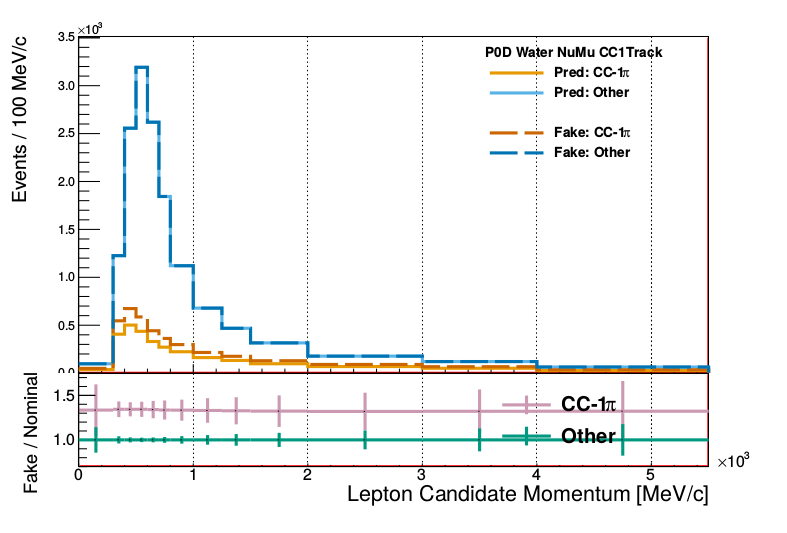
\includegraphics[height=0.4\textheight]{Chapters/Figures/Validation/CA5Variation/NuMu1Trk}
\par\end{centering}
}
\par\end{centering}
\begin{centering}
\subfloat[$\protect\numu$ in FHC Mode CC N-Tracks]{\begin{centering}
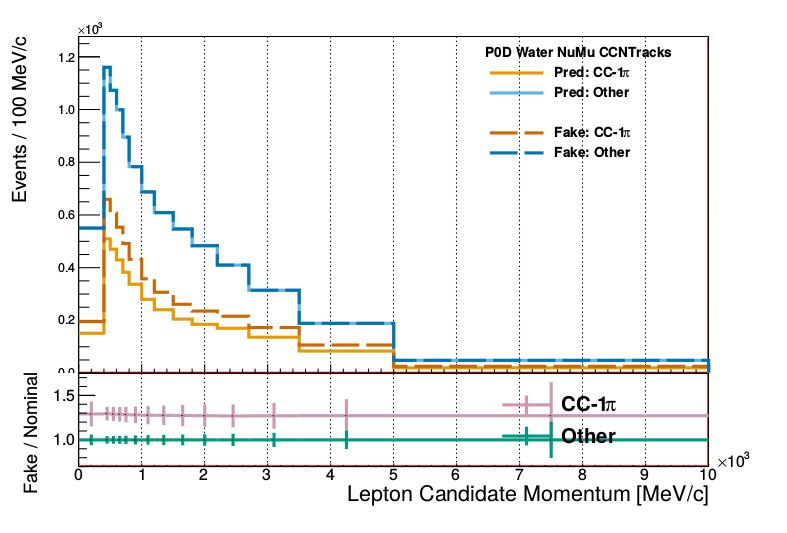
\includegraphics[height=0.4\textheight]{Chapters/Figures/Validation/CA5Variation/NuMuNTrks}
\par\end{centering}
}
\par\end{centering}
\caption[Lepton Candidate Momentum Distributions in the Single Pion Event Rate
Variation Fake Data Set]{Lepton candidate momentum distributions in the Single Pion Event Rate
Variation fake data set. The nominal MC and fake data predictions
are shown as solid and dashed lines, respectively. True CC-$1\pi$
events are differentiated from all other interactions to illustrate
the event scaling applied. A ratio plot of CC-$1\pi$ events to all
other interaction events shown beneath each main histogram. \label{fig:lepton-moentum-single-pion-fake-data}}
\end{figure}
\begin{figure}
\begin{centering}
\subfloat[$\protect\numubar$ in RHC Mode CC 1-Track]{\begin{centering}
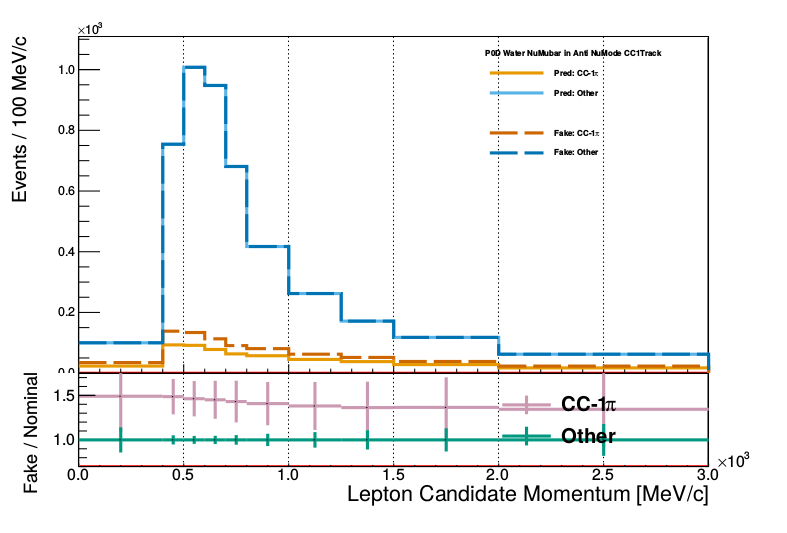
\includegraphics[width=0.48\textwidth]{Chapters/Figures/Validation/CA5Variation/ANuMuRHC1Trk}
\par\end{centering}
}\subfloat[$\protect\numubar$ in RHC Mode CC N-Tracks]{\begin{centering}
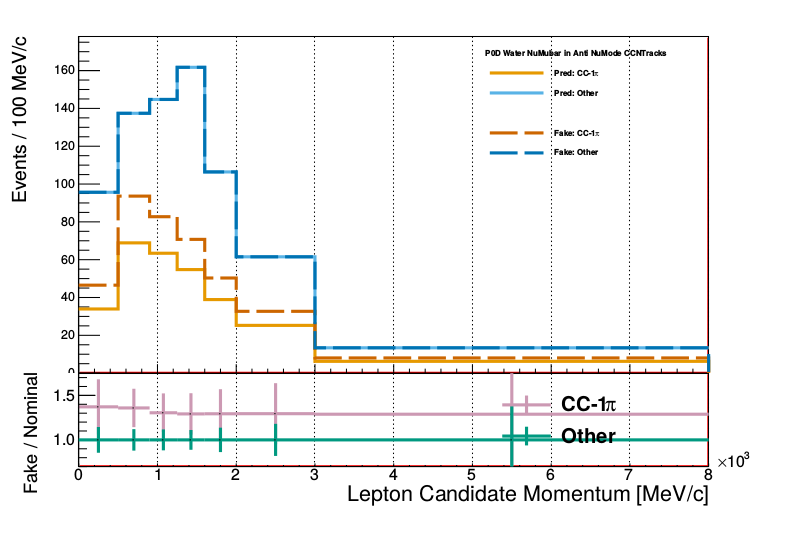
\includegraphics[width=0.48\textwidth]{Chapters/Figures/Validation/CA5Variation/ANuMuRHCNTrks}
\par\end{centering}
}
\par\end{centering}
\begin{centering}
\subfloat[$\protect\numu$ in RHC Mode CC 1-Track]{\begin{centering}
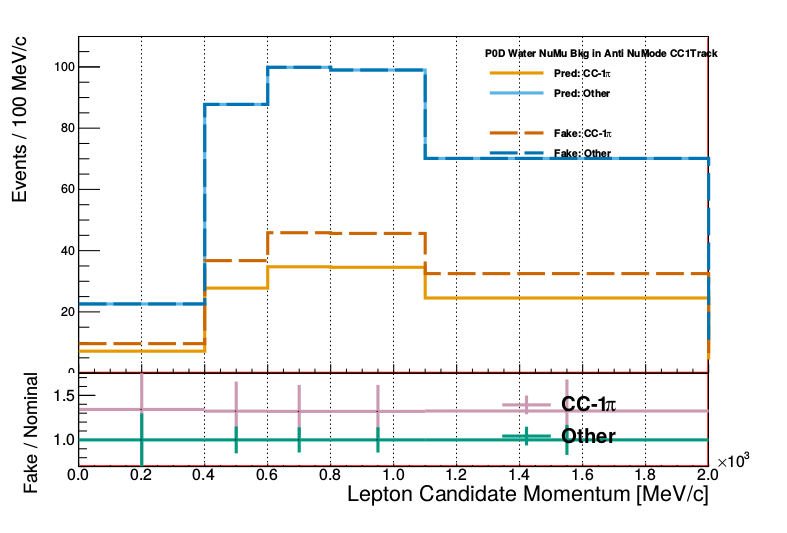
\includegraphics[width=0.48\textwidth]{Chapters/Figures/Validation/CA5Variation/NuMuRHC1Trk}
\par\end{centering}
}\subfloat[$\protect\numu$ in RHC Mode CC N-Tracks]{\begin{centering}
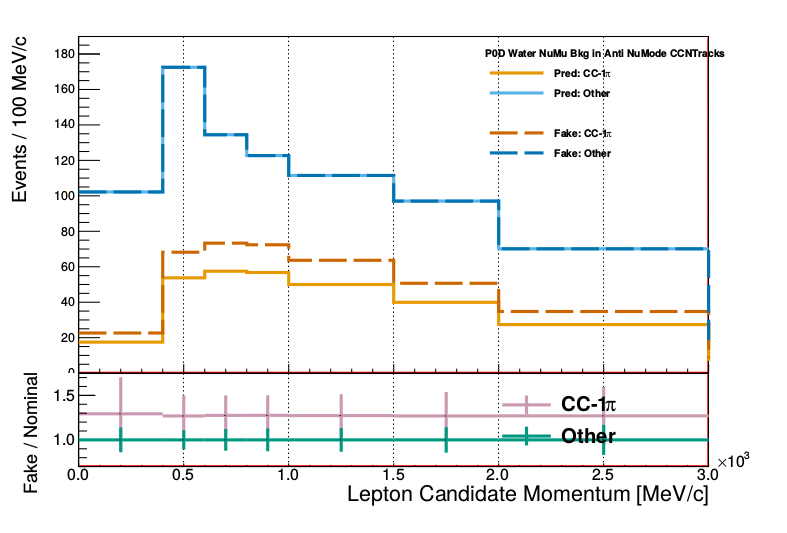
\includegraphics[width=0.48\textwidth]{Chapters/Figures/Validation/CA5Variation/NuMuRHCNTrks}
\par\end{centering}
}
\par\end{centering}
\caption[Lepton Candidate Momentum Distributions in the Single Pion Event Rate
Variation Fake Data Set (Continued)]{Lepton candidate momentum distributions in the Single Pion Event Rate
Variation fake data set (continued). The nominal MC and fake data
predictions are shown as solid and dashed lines, respectively. True
CC-$1\pi$ events are differentiated from all other interactions to
illustrate the event scaling applied. A ratio plot of CC-$1\pi$ events
to all other interaction events shown beneath each main histogram.
\label{fig:lepton-moentum-single-pion-fake-data-1}}
\end{figure}

This fake data test will help us understand the BANFF fit response
due to poor data matching with a cross section model. The ideal result
of this test is that the postfit value of $C_{A}^{5}$ is increased
by +25\% and all other parameters are unchanged like the results seen
in Appendix \prettyref{app:NSigmaVariations}. However, this is not
a realistic expectation given that there are no dedicated CC-$1\pi$
samples, thus the sensitivity to CC-$1\pi$ parameters is expected
to be small. In particular, the $C_{A}^{5}$ and $M_{A}^{\text{Res}}$
parameters are strongly anticorrelated with one another, meaning that
these parameters will be forced to shift in opposite directions. From
our intuition gained in the first fake data fit, we can expect non-CC-$1\pi$
parameters to vary especially groups of flux parameters together.

The postfit results for this fake data set are shown in \prettyref{fig:Postfit-single-pion-fake-data}.
We observe that the CC-$1\pi$ parameter $C_{A}^{5}$ increased by
\textasciitilde 10\%, but this is not enough to account for the input
fake data shift. We also notice that due to anticorrelations, $M_{A}^{\text{Res}}$
was decreased by several percent. What the fit prefers is to increase
the isospin=$\nicefrac{1}{2}$ background, 2p2h normalization, and
all the flux parameters. As seen in the first fake data set, we see
that in the presence of nonphysical variations to the physics, the
fit prefers to spread out variations among the other parameters. However,
this time the variations are shared among both the flux and cross
section parameters.

\begin{figure}
\begin{centering}
\subfloat[ND280 FHC Flux]{\begin{centering}
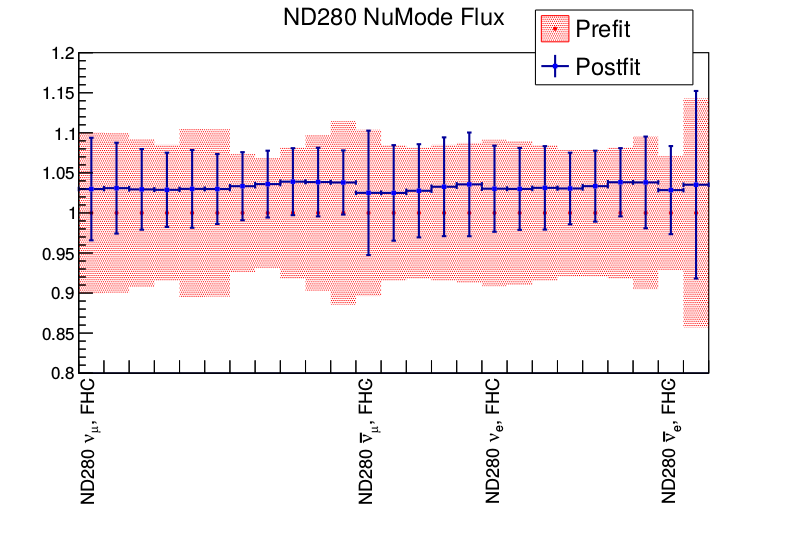
\includegraphics[width=0.48\textwidth]{Chapters/Figures/Validation/CA5Variation/ND280NuMu}
\par\end{centering}
}\subfloat[ND280 RHC Flux]{\begin{centering}
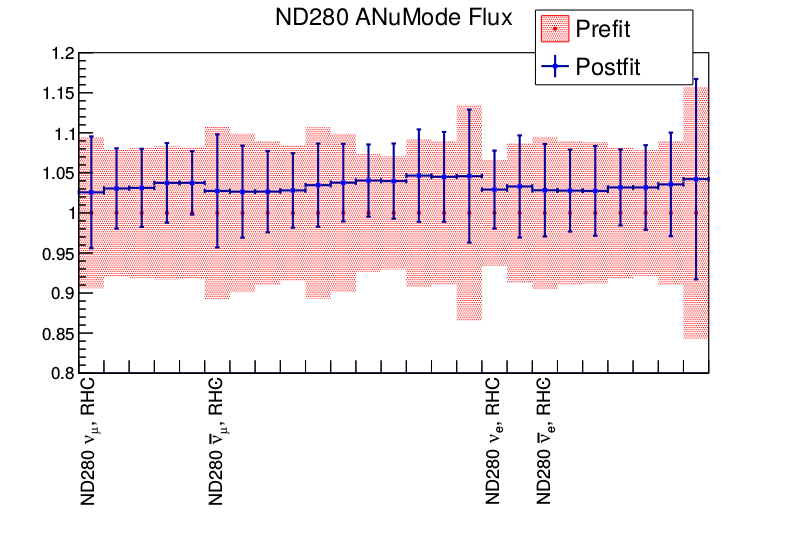
\includegraphics[width=0.48\textwidth]{Chapters/Figures/Validation/CA5Variation/ND280ANuMu}
\par\end{centering}
}
\par\end{centering}
\begin{centering}
\subfloat[FSI parameters]{\begin{centering}
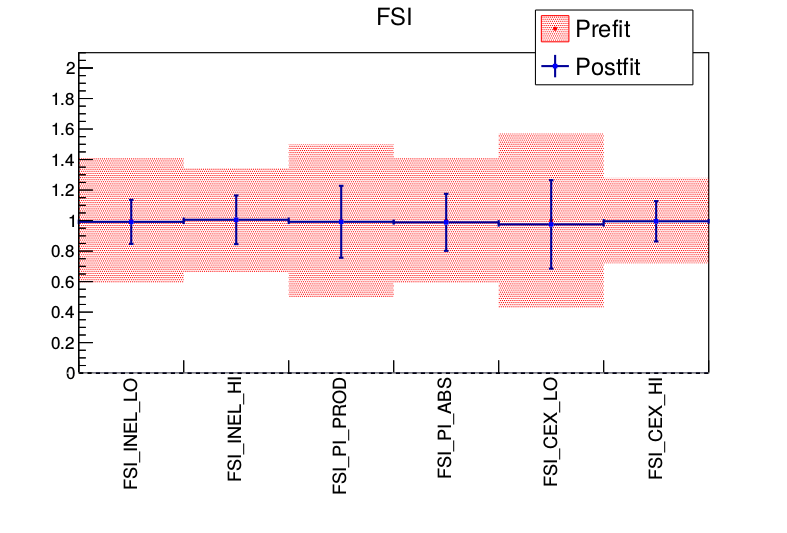
\includegraphics[width=0.48\textwidth]{Chapters/Figures/Validation/CA5Variation/FSI}
\par\end{centering}
}\subfloat[Cross section parameters]{\begin{centering}
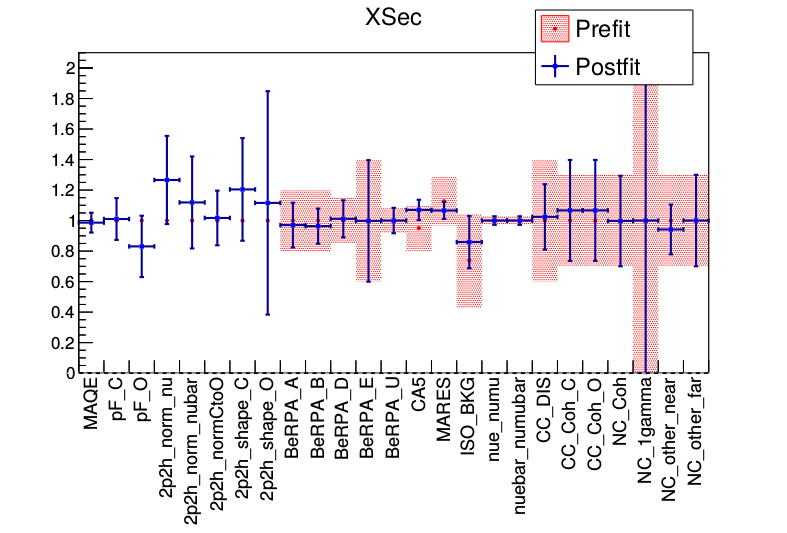
\includegraphics[width=0.48\textwidth]{Chapters/Figures/Validation/CA5Variation/XSec}
\par\end{centering}
}
\par\end{centering}
\caption[Postfit Parameters for the \texorpdfstring{$C_A^5$}{CA5} Fake Data
Fit]{Postfit parameters for the Single Pion Event Rate Variation fake data
fit. All the flux parameters in FHC are shown together and ordered
sequentially from left to right. The same is true the RHC flux.\label{fig:Postfit-single-pion-fake-data}}
\end{figure}


\section{Summary\label{sec:ValidationSummary}}

We have validated that the BANFF fit works and tested its robustness
in a variety of scenarios. We learned from the Asimov data set, which
is the T2K nominal MC corrected to data POT with fine tuning corrections,
in particular how the flux and cross section parameters affect the
samples. In the fake data sets, we saw the effect of the penalty terms
and how their correlations influence the fit. While more rigorous
tests could establish where biases exist, these limitations are beyond
the scope of this technote. What has been established is that sensible
fit results using the $\pod$ selections are possible. We will now
use the real $\pod$ data in the BANFF fit.
